 \documentclass{GlobalDocument}
\usepackage[landscape, top=0.5in, bottom=0.5in, left=2in, right=0.3in]{geometry}
\usepackage{subcaption} % for sub-figures
\usepackage{array}
\usepackage{pdfpages}
\usepackage{multirow}

\usepackage{multicol}

% Title Page
\title{
\includegraphics[width=0.5\textwidth]{images/title}\\Project Plan}
\author{\ourteam}

\begin{document}
\BgUsetrue % activates background (leave this off while working, it makes the compilation waaay slower)

\maketitle

\chapter{General Information}

\section{Version History}
\begin{tabular}{| p{0.2\textwidth} | p{0.2\textwidth} | p{0.5\textwidth} |}
  \hline
  Version Number & Date & Description \\
  \hline
  1 & 2015 September 11 & Initial project plan\\
  \hline
\end{tabular}


\section{Sign-off}
\begin{tabular}{| m{0.3\textwidth} | m{0.3\textwidth} | m{0.3\textwidth} |}
  \hline
  Name & Date & Signature \\
  \hline
  Ian Martin & \today & 
\includegraphics{images/ians}\\ 
  \hline
  Ryan Bluth & \today & \includegraphics{images/ryans}\\
  \hline
  Michael Hetman & \today & 
\includegraphics{images/michaels}\\
  \hline
  Sean LeBlanc & \today & \includegraphics{images/seans}\\
  \hline
  Emma Thurlow & \today & 
\includegraphics{images/emmas}\\
  \hline
  Catherine Wong & \today & 
\includegraphics{images/cats}\\
  \hline
\end{tabular}


\setcounter{secnumdepth}{3}
\linespread{1.0}
\setlength{\parskip}{0em}

\renewcommand*\contentsname{Table of Contents}
\tableofcontents

\listoffigures

\linespread{1.15}
\setlength{\parskip}{1.15em}
\normalsize

\chapter{Introduction}
For senior project, \ourteam{} plans to create a procedurally generated environment and narrative, full of strange and interesting characters to interact with. The goal of \ourgame{} is to provide players with a world of fantastical wonder that they can explore to their heart's content. In the game, the player will be a guest invited to the house party of the mysterious Mr. Omar Clean. After meeting Omar, the player is rudely interrupted by another strange man who strikes him on the head with a large cylindrical object. With Omar lying dead on the ground, the assailant turns his focus to the player and quickly knocks them out. Moments later, the player is awoken by another party-goer who reveals themselves to be a detective investigating the recently-deceased host. Now the player must explore the party, navigating the many strange social situations of the guests, while finding clues as to who the assailant was and unravelling the mysteries of the house. From there, the narrative unfolds further and further into a dimension-spanning science fiction epic. The player will experience this story through multiple short playthroughs. Each time, new core story elements will be introduced to the player, while the structure of each playthrough will be relatively similar. As the game's environment is procedurally generated, all the minor story elements will be unique for each playthrough as well. Who really is Omar Clean? What is actually going on at this \textit{"Party, Darling?"}

% Challenges stuff
%Although the process of procedurally generating content will allow the team to produce a larger variety of assets in a shorter amount of time, providing each player with a unique experience, the generation process must be efficient and produce high quality results in order for them to be up to par with individually crafted assets. \ourteam{} is also continuing the development of an in-house open source engine for this project. While this means that the developers will be intimately familiar with the engine, and the engine will be customizable to fit the needs of the project, it may take more time than estimated to solve unforeseen problems that other engines have already addressed. Another challenge will be that writing a narrative based in an ever-changing setting is difficult, especially when \ourteam{} hopes for the story to hold players until the end of the game. Marketing of the project will also need to be taken care of. As an independent development team, \ourteam{} will only have social media and networking events with which to promote our game and engine. This means that the management of these accounts will take time away from development to go out and show off the product at early stages. Despite the additional effort, this will allow the team to receive feedback and criticism which can be taken into account in improving \ourgame{}. One thing that \ourteam{} will need to be constantly aware of is that, due to the fluid nature of the project, it will be difficult to prevent feature-creep, resulting in an unmanageably large scope. In order to avoid this, \ourteam{} must be wary of arbitrarily proposed features and only include those which are absolutely necessary for the success of the project.

%Here you will have a general introduction to your project, main idea, high-level goals, and challenges.

%Goal: The purpose toward which an endeavour is directed.

%Main Idea:

%-For our senior project,plan to create a procedurally generated world and narrative, full of strange and interesting characters to interact with.
%High-Level Goals:

%- The goal of the Sweetheart Squad is to provide players with a world full of fantastical wonder that they can explore to their hearts content. 

%Challenges:

%- Although the process of procedurally generating content will allow the team to produce a larger variety of assets in a shorter amount of time, providing each player with a unique experience, the generation process must be efficient and produce high quality results in order for them to be up to par with hand-crafted assets.

%- A challenge we are undertaking is continuing the development of an in-house open source engine for this project. While this means that our developers are intimately familiar with the engine, and will allow us to customize the engine to fit the needs of the project, it may take more time than estimated to solve unforeseen problems that other engines have already addressed.

%- One challenge we will face is that writing a narrative based in a setting that is ever-changing is difficult, especially when we hope the story will have the ability to hold players until the end of the story.

%- Another challenge is the marketing of our project. As an independent development team, we only have social media and networking events with which to promote our game and engine. This means that we have to manage these accounts and take time away from development to go out and show off our products at early stages. Despite the additional effort, this will allow us to receive feedback and criticism which can be taken into account.

%- Due to the fluid nature of the project, the scope seems to constantly increase. During development, we will have to ensure that we do not bite off more than we can chew and to cut un-important proposed features when necessary.


\chapter{Main Objective}
\ourteam{} hopes to create a fully functional game that is procedurally generated, providing unique experiences to all players inside a linear narrative. The main components of the project that \ourteam{} hopes to include are a fully capable open-source engine, a scenario editor, an engrossing narrative, and a procedural generation system which outputs rooms, furniture, characters, and audio.



\chapter{Requirements and Features}
Each feature has been given a priority rating based on their relevance to \ourteam{}'s vision for \ourgame{}. The different priority ratings are as follows:
\begin{description}
\item[Essential]{- Features which are the bare minimum required for \ourteam{} to create the basic structure of \ourgame{}. These features will not be dropped.}
\item[Planned]{- Features which are required for \ourteam{} to fully realize the intended vision of \ourgame{}. Dropping any of these features will have a significant effect on the final product, but would not render the game unplayable.}
\item[Optional]{- Features which would enhance and build upon the main vision, but can be dropped or changed without significantly affecting the core experience of \ourgame{}.}
\end{description}

\section {Gameplay Features}
\subsection{Point-of-View and Navigation [Planned]}
Players of \ourgame{} will experience the 3D world from a first-person point-of-view. This means that the player will need to have control over a camera which simulates their own perspective and restrictions. As a result, this will be a perspective camera with an approximately 90 degree field of view which can be oriented in any direction, controlled by mouse and/or analog stick movement. It will be positioned at approximately eye level, and the player will be given control over two-dimensional movement in the horizontal plane. The movement of the camera will be controlled by standard keyboard controls (WASD) and/or game controller analog sticks.

\subsection{Rooms and Exploration [Essential]}
The game environment will be composed of a configuration of rooms that the player will be able to explore. These connections between different rooms will be represented as door items which the player can interact with in order to traverse the map. An example of a door in-game can be seen in Figure~\ref{fig:door}. The generation algorithm for the game environment is described in detail in Section~\ref{sec:room_generation}.

\begin{figure}[htb]
\centering
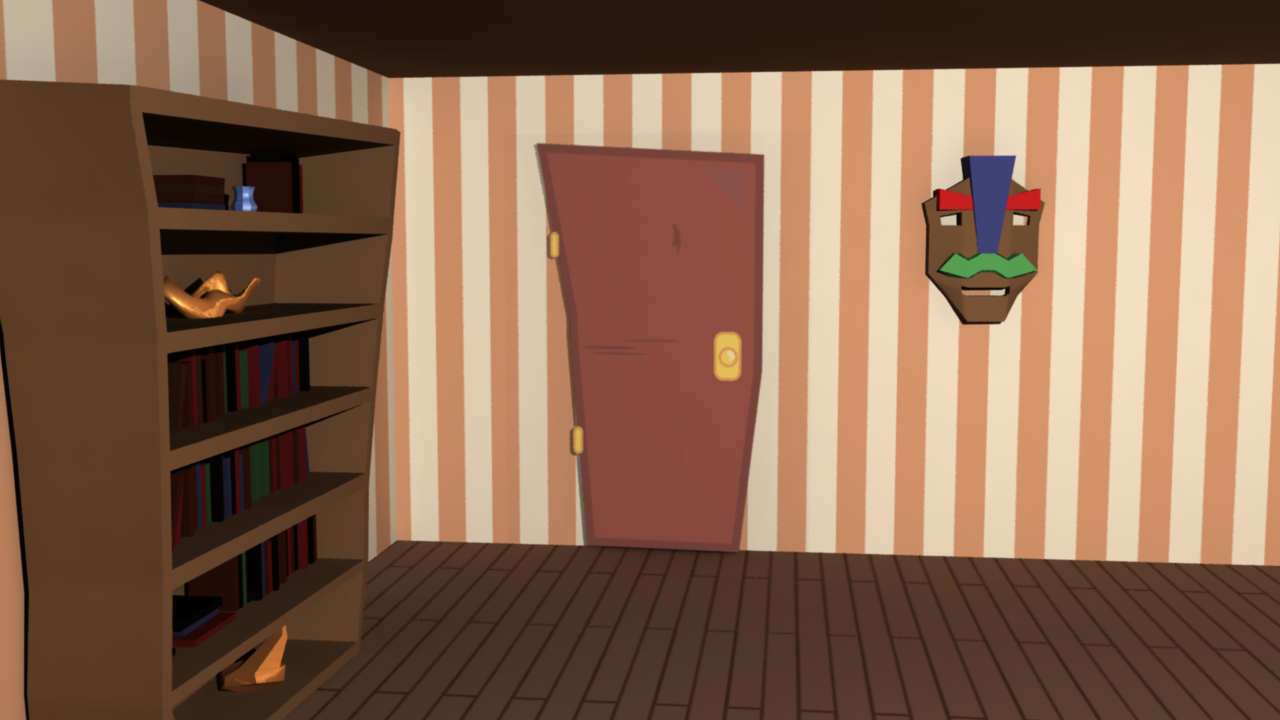
\includegraphics[width=0.6\textwidth]{images/Door2}
\caption{Interactive door object}
\label{fig:door}
\end{figure}


\subsection{Character Interaction [planned]}
\label{sec:character_interaction}
While exploring, the player may focus on a non-player character (NPC) by looking at them from within a certain distance. This will present the player with three options: \textbf{Talk}, \textbf{Recruit}, and \textbf{Yell}. The outcome of these systems will allow the player to progress through the storyline in various ways. 

\subsubsection{Talk [planned]}
The Talk option will begin a conversation with the focused NPC. There are two types of conversations the player can have with NPCs in \ourgame{}.

The first type of conversation will be those assigned to only plot-specific characters. While conversing with a plot-specific character, player movement will be disabled and the camera will zoom in on the NPC. As the character speaks, dialogue is shown in a speech bubble at the top of the screen. These characters will usually have more than one line of dialogue, so the player may click the speech bubble at any time to progress the conversation. During the conversation, the player may occasionally be prompted to choose something to say from a list of options. Each option will be shown as a speech bubble at the bottom of the screen. This interface will be similar to the main interaction UI described in Section~\ref{sec:interaction_UI}. All elements of the conversation will be written in the scenario files, and may include triggers for changing player state, affecting the game world, or initiating the yelling contests described in Section~\ref{sec:yelling}.

The second type of conversation triggers when the focused NPC is in a \textbf{non-speaking} state. While in a non-speaking state, the character will speak a single line, shown as text in a speech bubble above their head. This can be seen in Figure~\ref{fig:speech_bubble}. Characters are considered to be in a non-speaking state if they are not involved with any plot events, if they are upset with the player, or they are busy with a particular action. For most characters, this single line will be procedurally generated or selected randomly from a list of pre-written lines. For plot-specific characters, a specific line of dialogue can be written into their scenario. In order to provide variety, multiple lines may exist for a single character and will be cycled through on multiple interactions.

\begin{figure}
  \begin{subfigure}{.45\textwidth}
    \centering
    \includegraphics[width=.9\linewidth]{images/item_held_npc}
    \caption{Character without dialogue}
	\label{fig:speech_bubble}
  \end{subfigure}%
  \begin{subfigure}{.45\textwidth}
    \centering
    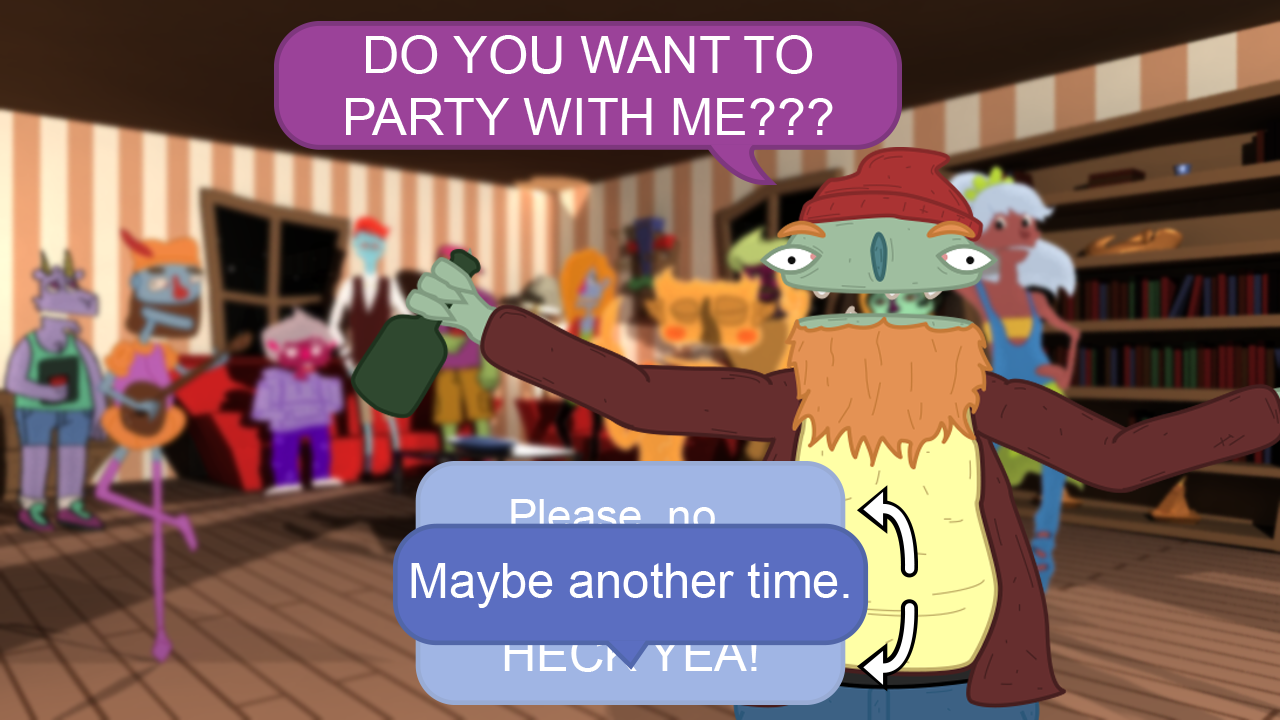
\includegraphics[width=.9\linewidth]{images/ConversationUI}
    \caption{Character with dialogue}
	\label{fig:dialogue}
  \end{subfigure}%
  \caption{Characters reacting to talk interactions}
\end{figure}

\subsubsection{Recruit [Planned]}
Throughout the game, players will have the ability to ask NPCs to follow them by selecting the Recruit option. The character will agree to follow the player if their \textbf{friendship rating} is high enough. Interacting with characters and completing scenario events will increase or decrease the player's friendship rating with certain characters.

In the yelling mini-game described in Section~\ref{sec:yelling}, followers act as extra lives for the player. When a follower is expended in battle, they will stop following the player. The player can also lose a follower if that follower's friendship rating falls below a certain threshold. The player can lower a follower's friendship rating by making narrative choices that follower doesn't agree with, or starting yelling battles with NPCs aligned with the follower.

\subsubsection{Yell [Planned]}
\label{sec:yelling}
Yelling contests may be initiated in one of two ways: the player may trigger one by intentionally selecting the Yell option while interacting with a character, or they may be triggered by NPCs as part of a scripted sequence. The interaction of a yelling contest can be roughly described as a tug-of-war between the two sides of the conversation, wherein a victor is decided when one side has maintained control for a sustained period of time.

When an NPC is in control of a contest, they will bombard the player with continuous insults, each one tipping the scale towards the NPC's victory. This can be seen in Figure~\ref{fig:yelling_contest_offense}. In order to gain control, the player is given the opportunity to \textbf{interject} when the NPC pauses at the end of a thought or a sentence. If the player successfully interjects the opposing NPC mid-insult, shown in Figure~\ref{fig:yelling_contest_interject}, they will be put on the defensive and tasked with maintaining control. While in control of a contest, the player will be presented a partial insult with two possible conclusions. One of the presented options will complete the insult, and the other will result in an ineffective insult; an example is given in Figure~\ref{fig:yelling_contest_defense}. The player has a limited time to choose the correct conclusion. If the player chooses incorrectly or their time runs out, the opposing NPC will interject and regain control. If the player chooses correctly, they will tip the scale towards their victory and be presented with another partial insult to complete. The difficulty of maintaining control will increase linearly with the time spent in control by reducing the length of time given to the player to complete insults. 

After each battle, the player loses a little bit of their \textbf{voice}. As the player loses their voice more and more, they will have less time to complete their insults in the yelling contest. The player can heal themselves by drinking beverages they find around the party. Implementing this limitation adds an extra level of strategy to the yelling contests, and requires the player to be mindful of how they use the Yell option.

\begin{figure}[htb]

\begin{subfigure}{.33\textwidth}
\centering
\includegraphics[width=.9\linewidth]{images/Yelling_UI_Interupt}
\caption{NPC in control - player must attempt to interject at highlighted pauses}
\label{fig:yelling_contest_offense}
\end{subfigure}%
\begin{subfigure}{.33\textwidth}
\centering
\includegraphics[width=.9\linewidth]{images/Yelling_UI_Interupted}
\caption{Successful interjection by player}
\label{fig:yelling_contest_interject}
\end{subfigure}%
\begin{subfigure}{.33\textwidth}
\centering
\includegraphics[width=.9\linewidth]{images/Yelling_UI_Burn}
\caption{Player in control - player must choose insults instead of compliments while maintaining the rhythm}
\label{fig:yelling_contest_defense}

\end{subfigure}%
\caption{Yelling Contest mockups}
\label{fig:yelling_contest}
\end{figure}

\subsection{Items [Planned]}
\subsubsection{States [Planned]}

Items may exist in one of three distinct states:
\begin{description}
\item[Static]{- Items that appear in the environment.}
\item[Held]{- Items that are held, either by the player or by an NPC.}
\item[Stored]{- Items that are kept in the inventory of the player or of an NPC.}
\end{description}

\subsubsection{Representation [Planned]}
Each item in \ourgame{} will be represented by a single 2D sprite. The specifics of how item sprites are rendered is dependent on a given item's current state. Static items will be rendered onto a single 3D polygon entity within the game world. When held items belong to a non-player character, the item sprite will be rendered on top of one of their hands. When items are held by the player character, the item sprite will be rendered at the bottom of the screen inside the player's bubble UI. Items stored by non-player characters will not be rendered, and items stored by the player character will be shown in a 2D inventory screen, described in Section~\ref{sec:inventory}. 

\begin{figure}[htb]
  \begin{subfigure}{.24\textwidth}
    \centering
    \includegraphics[width=.9\linewidth]{images/swordonTable}
    \caption{Item leaning on a table.}
  \end{subfigure}%
  \begin{subfigure}{.24\textwidth}
    \centering
    \includegraphics[width=.9\linewidth]{images/item_held_npc}
    \caption{Item held by NPC}
  \end{subfigure}%
  \begin{subfigure}{.24\textwidth}
    \centering
    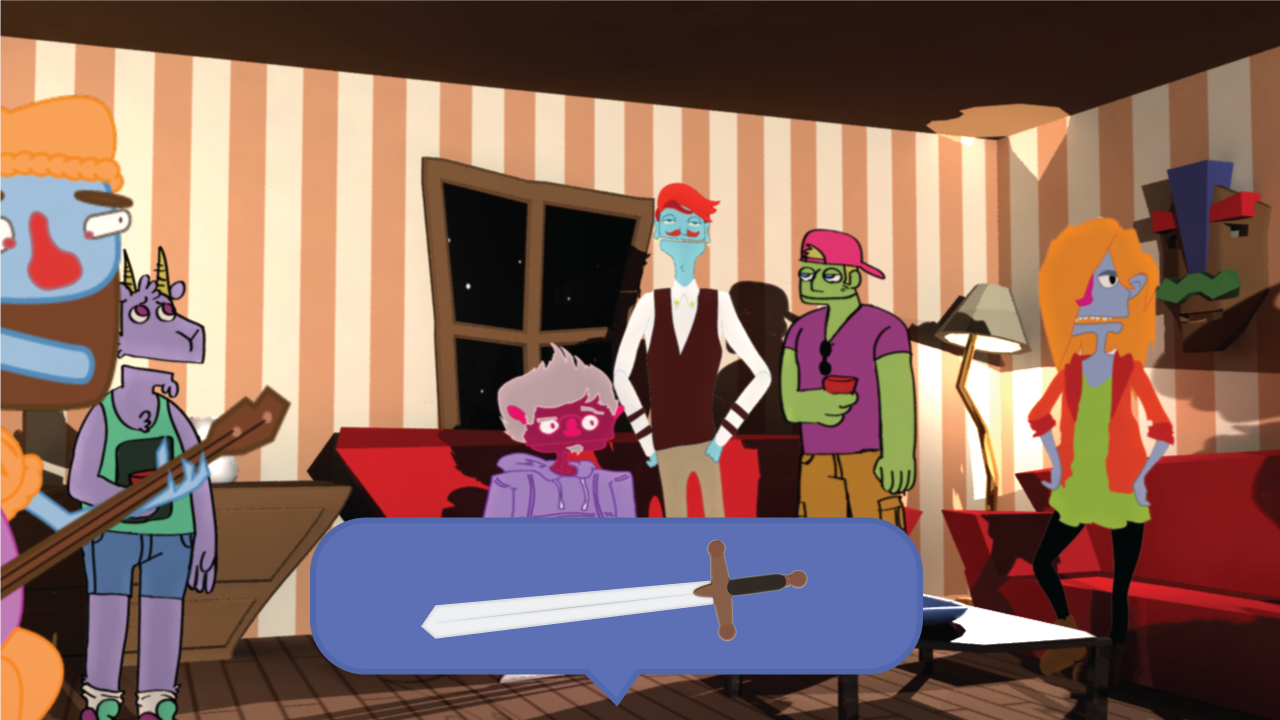
\includegraphics[width=.9\linewidth]{images/CharacterItem}
    \caption{Item held by player}
  \end{subfigure}%
  \begin{subfigure}{.24\textwidth}
    \centering
    \includegraphics[width=.9\linewidth]{images/itemInventory}
    \caption{Item stored by player}
  \end{subfigure}%
  \caption{Single item in different states}
\end{figure}

\subsubsection{Interaction [Planned]}
\label{sec:item_interaction}
When the player is empty-handed, they can interact with a static item. The item is removed from the world and replaces the player's cursor. This changes the item's state to Held, and changes its owner to the player. While the item is being held, the player is given two options: \textbf{Use}, and \textbf{Drop}. The Drop option will revert the item to its static state and remove ownership, placing it back into the world at the player's position. The Use option is context-sensitive, and will change based on what the player is currently looking at. If the player is focusing on a non-player character, the Use option will trigger an interaction between the held item and the NPC. If the player is not looking at an object with which they can use the item, the Use option will instead trigger an interaction between the item and the player themselves.

Generic usable items will affect the statistics involved in yelling contests, described in Section~\ref{sec:yelling}, and will include beverages, as well as food products such as cupcakes, cocktail wieners, and other finger-food. Specific usable items will be defined in scenarios.


\subsection{Scenarios [Essential]}
A \textbf{scenario} in \ourgame{} is a package defining content for \ourgame{}. When talking to an NPC involved in a scenario, the player may be presented with a task. This task may involve finding an item, talking to another character, gaining a certain follower, or winning a yelling contest. Upon completing the task, the player often becomes friends with one or more NPCs involved in the scenario, meaning those NPcs can be recruited as followers by the player. The player may also receive an item that will assist them in another scenario, or an item that will help them in a yelling contest. Completing scenarios will not always be beneficial, as they may cause followers to leave if they do not like the outcome.

By completing scenarios, the player can make many friends at the party. Some scenarios will not be available to the player unless they have a certain number of friends. Making friends with specific characters can help the player in certain scenarios and also unlock new rooms in the house.


\section{UI Features}
\subsection{Interaction UI [Planned]}
\label{sec:interaction_UI}
The main interaction UI used throughout \ourgame{} will be placed at the bottom of the screen and will be present options to the player character in thought bubbles. In order to change their selection, the player may use the mouse's scrollwheel or use the directional keys on a keyboard or controller.

\begin{figure}[htb]
  \begin{subfigure}{.48\textwidth}
    \centering
    \includegraphics[width=.9\linewidth]{images/newNPCInteraction}
    \caption{NPC Interactions}
  \end{subfigure}%
  \begin{subfigure}{.48\textwidth}
    \centering
    \includegraphics[width=.9\linewidth]{images/UseItem}
    \caption{Item Interactions}
  \end{subfigure}
  \caption{Thought bubble interaction UI}
  \label{fig:interaction_UI}
\end{figure}

These thought bubbles will be context sensitive. In Figure~\ref{fig:interaction_UI}, the player is looking at an NPC, so the thought bubbles include the options described in Section~\ref{sec:character_interaction}. When the player is holding an item, the thought bubbles will include the options described in Section~\ref{sec:item_interaction}.


\subsection{Inventory [Optional]}
\label{sec:inventory}
As players will typically come across many different items in a single run, \ourgame{} will have an inventory system which allows the player to store these items for later use. This inventory will be represented as a backpack, which the player may open by pressing the TAB key. When opened, an interface is shown in which all of the player's currently stored items are shown inside a 2D representation of a backpack's outline, as shown in Figure~\ref{fig:inventory}. While the player is holding an item with the mouse cursor, that item can be placed into the backpack by clicking anywhere within the backpack's outline. This causes the item to be placed in the backpack at the mouse's position, and changes the item's state to Stored. Similarly, items may be taken out of the backpack by clicking on them, as long as the player is not already holding an item. When the player is empty-handed, clicking on an item in the backpack causes the item to be picked up, and changes the item's state to Held. The player can then press the TAB key to close the inventory, and can now use that Held item within the game world.

\begin{figure}[htb]
\centering
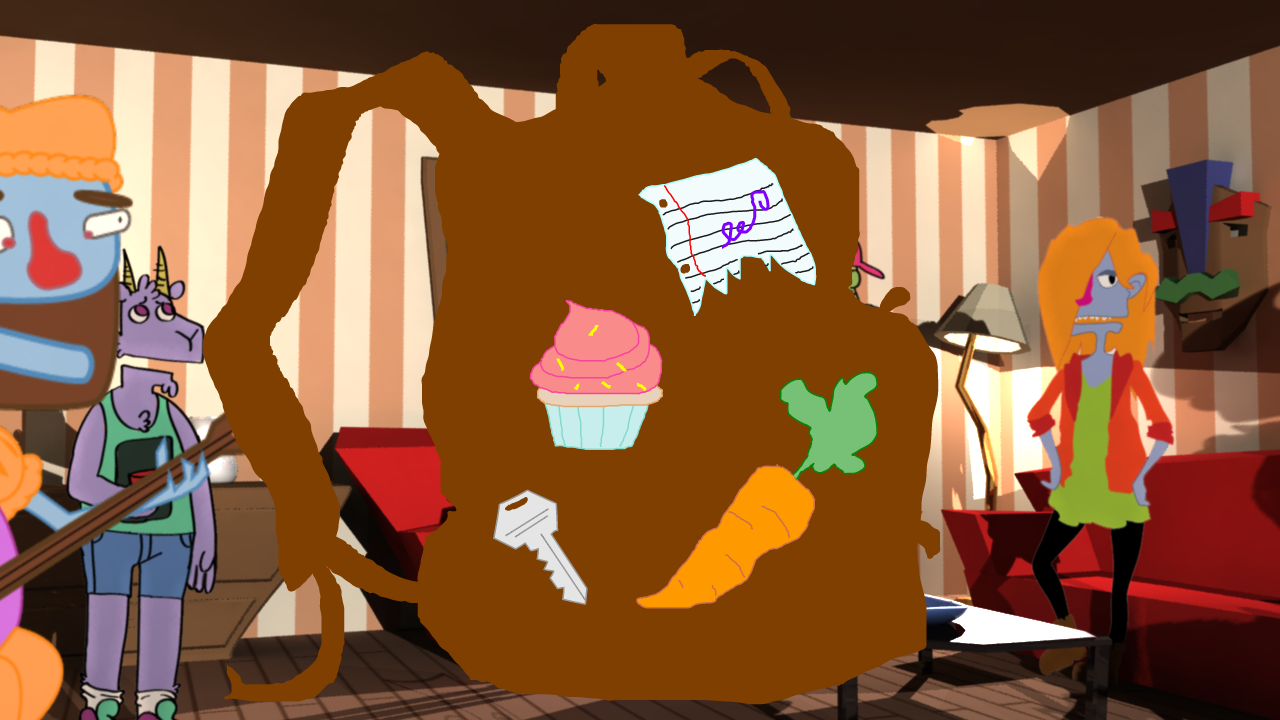
\includegraphics[width=.5\linewidth]{images/UI_inventory}
\caption{Player's Inventory}
\label{fig:inventory}
\end{figure}

\subsection{Menu [Essential]}

The main menu of \ourgame{} will include an option to play the game, an option to change certain settings in the game, and an option to quit the game. The settings menu will include a number of features to allow the player to customize the application to suit their computer.

\subsubsection{Variable Resolution [Planned]}
As \ourgame{} is planned for release on PC, it must take into account that PC gamers often have different preferences when it comes to monitor resolution. At a minimum, the settings menu for a PC game must include multiple standard variations of the 16:9 aspect ratio (720p, 1080p, etc). To account for any situation, \ourgame{} must be capable of detecting the different video modes available at runtime and present these to the player as options in the menu. When the player selects a new resolution, the resize data must be forwarded to the engine in order to maintain the field-of-view, and the out-of-date OpenGL context must be destroyed and replaced with a new one.

\subsubsection{Multiple Monitor Support [Optional]}
Although a standard PC environment can be assumed to have one monitor, it is not uncommon for PC gamers to have two or three monitors for a single computer. In these situations, it is often desirable for the player to be able to display fullscreen applications on a monitor which is not seen as the primary monitor by the system. As the default behaviour for a fullscreen application is to use the primary monitor, \ourgame{} will have to detect and display multiple fullscreen monitor options in the menu when available.

\subsubsection{Categorized Volume Controls [Optional]}
Although every system has a built-in master volume control, many players place value in the ability to customize volume on a per-application level. Additionally, volume in games is often further segmented into three categories: music, voice, and sound effects. These categories are typically presented in order to give players the freedom to tailor the experience to their own preferences. For example, some players prefer to complement games with their own music instead of the in-game background music, but would prefer if they could still hear the voice and sound effects when doing so.

In light of these standards and expectations, \ourgame{} will need to implement four volume controls: a master control, which affects the volume of every audio file played; a music control, which affects the volume of just the audio files containing background music; a voice control, which affects the volume of just the audio files used when characters are speaking; and a sound effects control, which affects the volume of the rest of the audio files used throughout the game. 

\section{Special Technologies}

\subsection{\ourengine{} [Essential]}
\ourengine{} is a game engine under development by \ourteam{}. \ourengine{} is publicly available on GitHub as an open source project which others may use and develop free of restrictions. Although \ourengine{} is still under development, it has been used by \ourteam{} to create a number of projects, some of which have been quite complex and rich with features. The benefit of using an in-house game engine is that \ourteam{} has full control over how it works, which allows the team to make changes quickly to existing systems or introduce new ones if needed. The fact that \ourengine{} has been developed internally also provides \ourteam{} with a deeper understanding of the core systems.

\subsubsection{Basic Nodes [Essential]}
\ourengine{} makes heavy use of inheritance to provide a set of base "Node" classes. When a more complex class is created for use in the engine, it will often inherit from one or more of these basic classes. The key node classes are described in Figure~\ref{fig:nodes}.

\begin{figure}[htb]
\begin{description}
\item[Node Updatable]{- An object which can be updated. The update function of Node Updatable is where any logic which needs to be run on a frame-by-frame basis will be placed. \ourengine{} performs an update each frame in which the current scene updates all of its children. The update function of Node Updatable takes a step object. This object contains information on how much time has passed since the last frame, what the target framerate is, and provides a ratio which may be used for correction if the previous frame did not meet that target.}

\item[Node Renderable]{- An object which can be rendered. Like update, \ourengine{} performs a render call each frame which draws all of the scene's children to the screen. The job of the render function of a Node Renderable derived class will be to pass OpenGL any variables specific to the object, and inform OpenGL to draw the object to the screen.}

\item[Node Loadable]{- An object which can be loaded and unloaded. This loading and unloading often pertains to the OpenGL context. An example of a loadable object would be a texture: in order to use a texture in the OpenGL context, a texture must be created on the GPU. Once the context is destroyed, so is the texture. This is where loading and unloading comes into play: When a Node Loadable is loaded, it should perform the operations required to interface with the GPU via OpenGL, and when it is unloaded, it should perform the required operations to clear itself from the GPU's memory.}

\item[Node Resource]{- A Node Loadable which can track references to itself. This allows for a single resource object such as a texture or mesh to be used across multiple objects without worry that it will be unexpectedly deleted. When deleting a Node Resource, the \textbf{decrementAndDelete} function is called instead of using the \textbf{delete} keyword. This function decrements the reference count and if it is zero then the object is deleted. This allows for proper memory management while using the object in multiple locations. In many cases, the use of Node Resource instances allows for a simple form of garbage collection, reducing the need for developers to spend time and effort attempting to account for complex memory management.}
\end{description}
\caption{\ourengine{} key node types}
\label{fig:nodes}
\end{figure}

One of the considerations that needs to be made in order to allow for the inheritance of multiple base Node classes is a resolution to the \textbf{diamond inheritance problem}. This problem arises when a class inherits from two derived classes of a single base class, and subsequent reference to base class member variables or functions become ambiguous. For a visual example, see Figure~\ref{fig:diamond_problem}. Since each of the Node classes described in Figure~\ref{fig:nodes} inherit from the same base class (i.e. Node), the diamond inheritance problem arises whenever a class must inherit from more than one of these Node classes.

\begin{figure}[htb]
\centering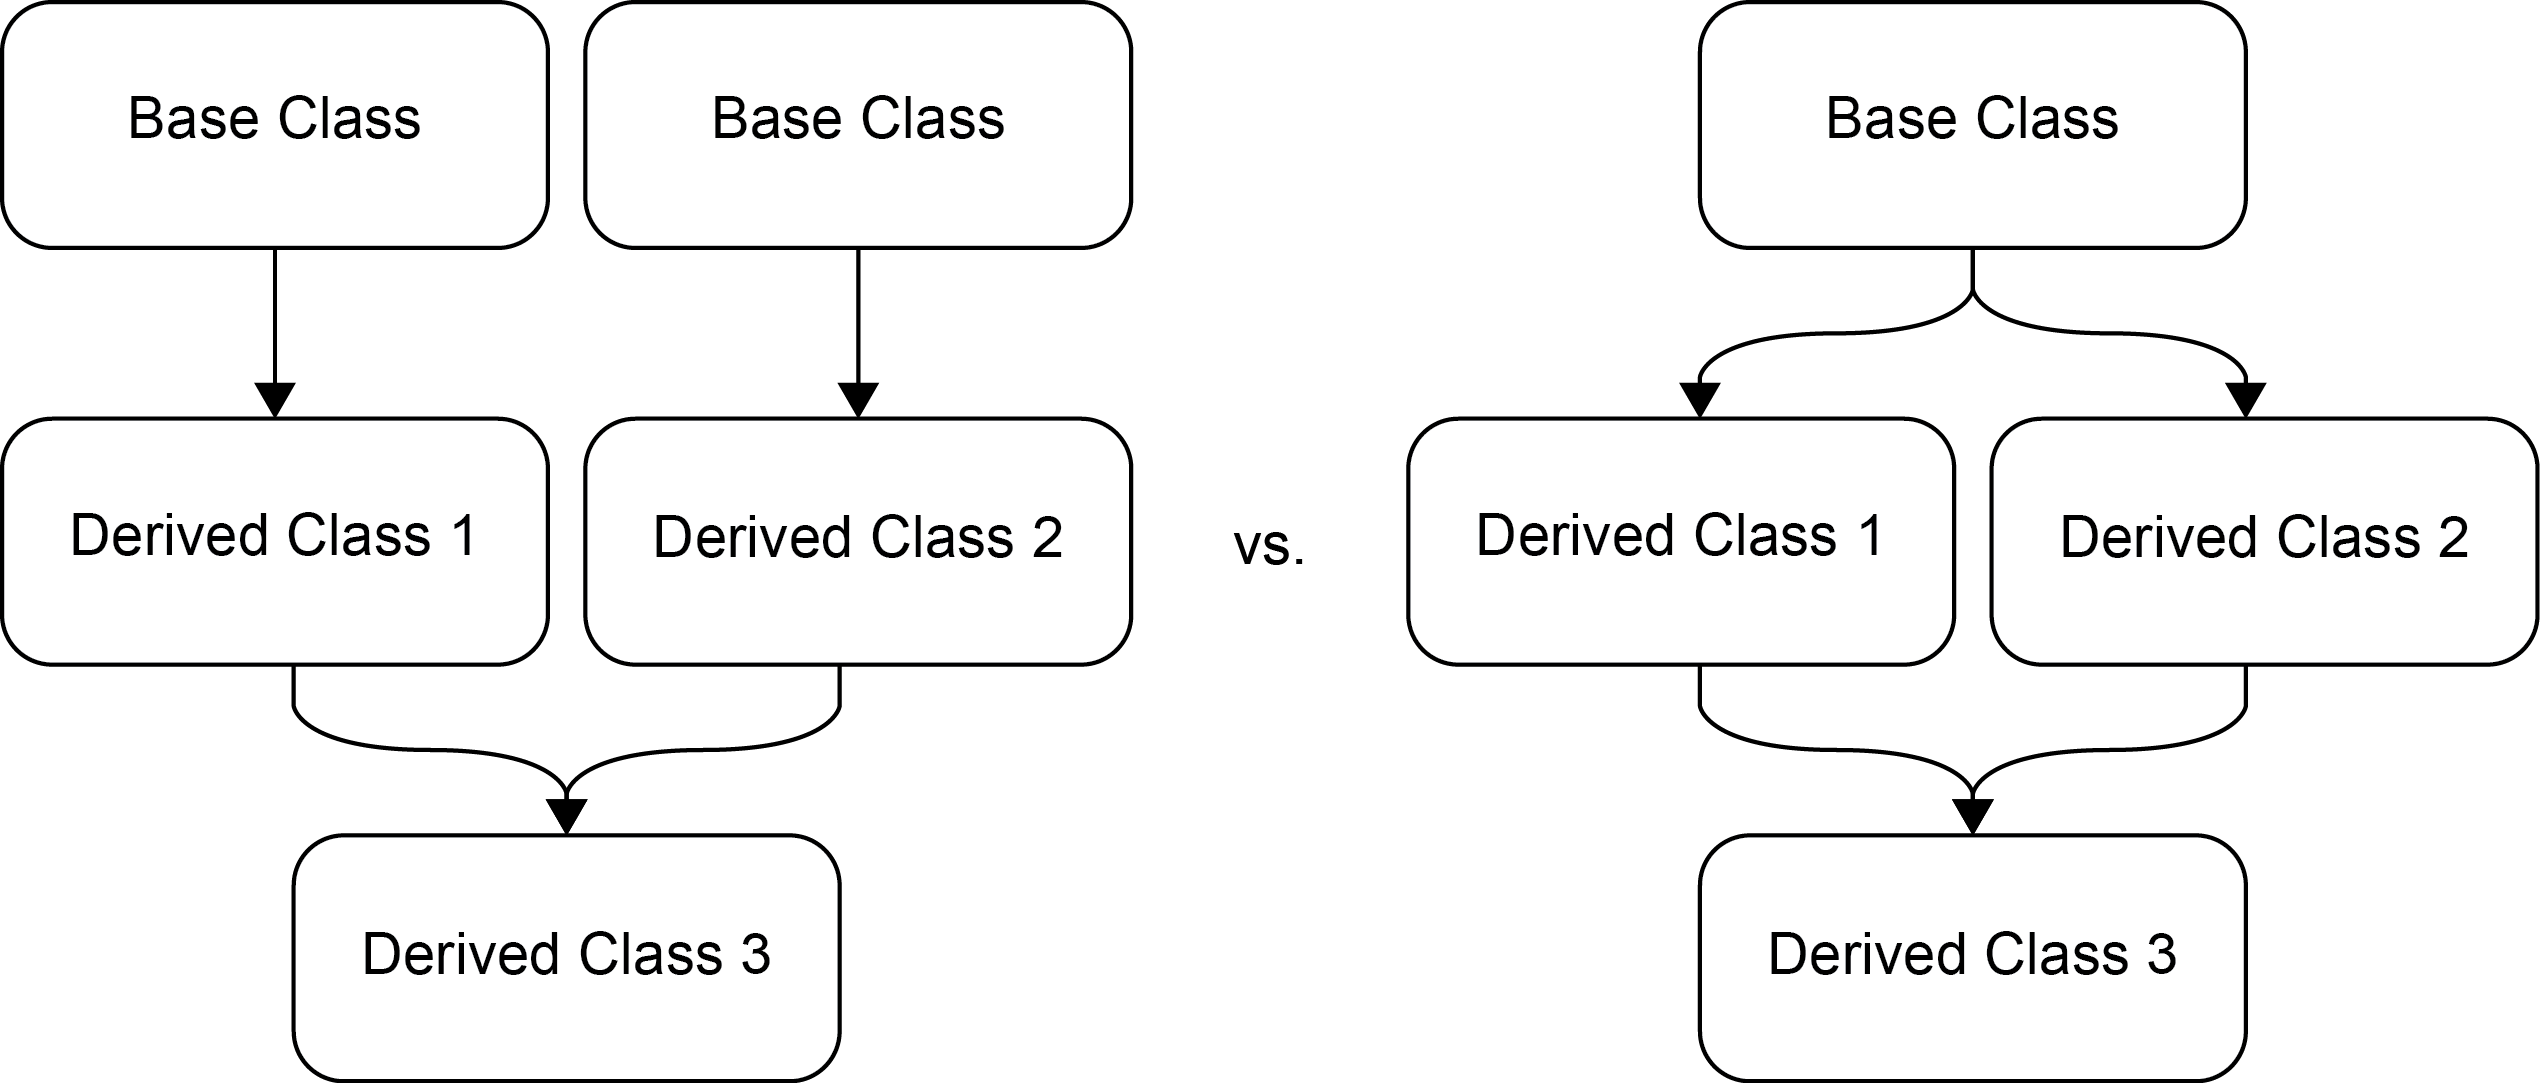
\includegraphics[width=0.5\textwidth]{images/diamond_inheritance}
\caption{Diamond Inheritance Problem}
\label{fig:diamond_problem}
\end{figure}

To solve the diamond inheritance problem, \ourengine{}'s base Node classes will use the concept of \textbf{virtual inheritance}. This will allow classes which inherit from a single base class multiple times through different derived classes to only instantiate a single instance of the multiply derived base class.

\subsubsection{Transform Hierarchy [essential]}
\ourengine{} implements a hierarchy system which acts as an implicit scene graph. The most important element in this system is the \textbf{Transform}. In \ourengine{} a Transform does a number of things, and is the only class which may have a direct list of children. A Transform object has a model matrix, which is a combination of three different transformation matrices: translation, rotation and scale. The model matrix is the product of these three matrices in a specific order, and is used on the GPU to calculate the world position of individual vertices being drawn to the screen. When a child is added to a Transform, any transformations applied to the parent Transform will also affect the child when it is drawn. If the child were also a Transform object, it may have its own transformations, which would then be applied to its own children. There is virtually no limit to the depth of this hierarchy, as it is implemented as a stack.

\subsubsection{Entitites [essential]}
Through \ourteam{}'s work on other projects, an initial limitation of \ourengine{} was quickly realized: because only Transform nodes may have a direct list of children, creating simple hierarchies of objects would require the game developer to instantiate many individual Transforms along with all of their game objects and then manually parent each object to a Transform and parent the Transforms to each other as needed. This process could lead to incredibly verbose and somewhat confusing code, and so the concept of Entities was introduced to make these situations easier for developers.

An Entity is an object within \ourengine{} which extends Node Updatable, Node Renderable, Node Loadable, and Node Child. In essence, this makes it a combination of every basic Node needed to create an interactive object which may use context-sensitive content and can be represented visually in the Scene. Additionally, the Entity class provides the member variable \textbf{childTransform}. This member variable stores a reference to a unique Transform instance which exists partially outside the standard Transform hierarchy and is intrinsically linked to the hierarchy of its encapsulating Entity. When the Scene iterates through to an Entity (such as during a call to update or render), the Entity will forward the call to its childTransform.

\subsubsection{UI [essential]}
Although the UI in \ourgame{} is fairly minimal, it will require a sophisticated UI rendering routine within the engine to ensure it is both extendable and aesthetically pleasing. The planned UI specifications are largely inspired by \ourteam{}'s web development experience and as such, shares many similarities with basic HTML and CSS.

One of the features which must be implemented into \ourengine{}'s UI specification is a content model which includes padding and margin. This content model will take advantage of the transform hierarchy which drives most of the rendering by representing both padding and margin as separate Transform nodes.

In order to give UI elements a consistent visual representation, each UI element will need to contain a simple mesh which represents its background. To make UI styling easier for developers, this mesh will need to include functionality for applying different colours, textures, and/or opacity. By default, container elements in the UI specification will have background meshes which are invisible. Should a developer wish to render these background meshes anyway, this option will be made available.

To account for standard mouse events, each UI element will need to extend a collider object. This collider object will be compared against the mouse position at each update and determine which mouse events to trigger. This comparison will take the form of a raycast against the collider, where the ray's start point is based on the camera's eye position and the position of the mouse and the ray's end point is based on the mouse position and a pre-defined ray length variable. Mouse events which will be triggered by this UI system are described in Figure~\ref{fig:mouse_events}.

\begin{figure}[htb]

\begin{description}
\item[In]{Triggered when the raycast against the collider is currently true AND the raycast against the collider was false in the previous update}
\item[Out]{Triggered when the raycast against the collider is currently false AND the raycast against the collider was true in the previous update}
\item[Down]{Triggered when the raycast against the collider is currently true AND the mouse is currently pressed AND the mouse was not pressed in the previous update}
\item[Up]{Triggered when the mouse is currently not pressed AND the mouse was pressed in the previous update}
\item[Click]{Triggered when the raycast against the collider is currently true AND the mouse is currently not pressed AND the mouse was pressed in the previous update}
\end{description}
\caption{\ourengine{} mouse events}
\label{fig:mouse_events}
\end{figure}

In order to create user interfaces a layout system will be required. The system must be capable of laying out items both horizontally and vertically. UI items added to a layout will stack as they are added to a layout and will respect the margins of the previous element. Nesting multiple linear layouts will allow for the creation of complex interfaces. 

The ability to add text of various styles will be a critical component of the UI system. On a technical level the layout of text will be achieved using the linear layout system. Each row of text will be created using a horizontal linear layout and these rows will be laid out vertically in order to create a text area. The styling of the text will be achieved through the use of specific shaders. 

This hierarchical approach to text and UI layout is very straightforward and is internally consistent with the rest of \ourengine{}'s scene hierarchy, however, the number of draw calls to individual Transforms will increase the computation time needed to render a scene. Textual data often involves hundreds if not thousands of individual characters, resulting in far too many draw calls for \ourengine{} to handle at a reasonable framerate for interactive media. In order to account for this inefficiency, UI rendering will use a combination of the process described above and offline rendering, wherein UI elements are first rendered to an offline texture, and then the offline texture is rendered to the screen in subsequent frames. The offline texture for a container element will only require updates when the child elements are visually updated, allowing most frames to render without having to process the individual elements.


\subsection{Procedural Generation}
\subsubsection{Rooms [Essential]}
\label{sec:room_generation}
At the start of each playthrough, a layout for \ourgame{}'s main environment -- the ever-changing mansion of the mysterious Mr. Omar Clean -- will be generated procedurally. The room generation algorithm starts by selecting approximately 10 scenarios from the game's database for use in the current playthrough. Once these scenarios have been selected, the various characters, items, and room specifications associated with those scenarios must be generated. Once these have been created, they will be grouped into bundles which may each be mapped to a single room at the end of the generation process. For example: one scenario may be defined such that it includes two characters and two room specifications, one of which is tagged with "bathroom". Each character must be placed in one of the specified rooms. A second scenario may be defined such that it includes a single item which must be placed within a container. A third scenario may be defined such that it includes a room specification with the "kitchen" tag. At this stage in the generation algorithm, two bundles will be created. The first bundle will include one room specification with the "kitchen" tag, one character, a single container, and the item; the second bundle will include a room specification with the "bathroom" tag and the other character. This example is visualized in Figure~\ref{fig:room_bundling}. Notably, two of the three rooms specified in the scenarios were merged, producing more potential interactions between the selected scenarios.

\begin{figure}[htb]
 \centering\includegraphics[width=.9\linewidth]{images/bundle_mockup}
  \caption{Visualization of room bundling}
  \label{fig:room_bundling}
\end{figure}


Once the scenario contents have been bundled, the layout of the house may be generated. To achieve this, a grid will be created, and subsections of the grid will be selected to create spaces for individual rooms. The size of the grid and individual rooms will be based on the specifications and required room content in each bundle. Inside each subsection, an image will be generated which represents the shape of the room. The room's walls will be created and placed depending on the contours calculated from the room-layout image's pixels. Examples of this procedural generation system can be seen in Figure~\ref{fig:room_generation_example}

\begin{figure}[htb]
 \centering
  \begin{subfigure}{.24\textwidth}
    \centering
    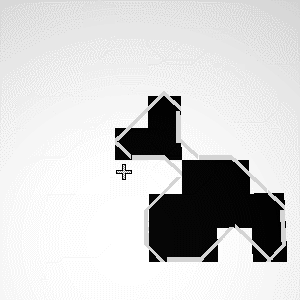
\includegraphics[width=.9\linewidth]{images/maps_0000}
  \end{subfigure}%
  \begin{subfigure}{.24\textwidth}
    \centering
    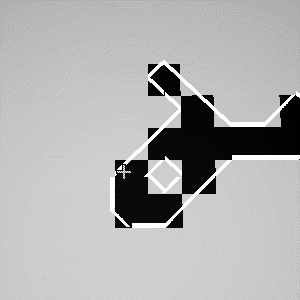
\includegraphics[width=.9\linewidth]{images/maps_0001}
  \end{subfigure}%
  \begin{subfigure}{.24\textwidth}
    \centering
    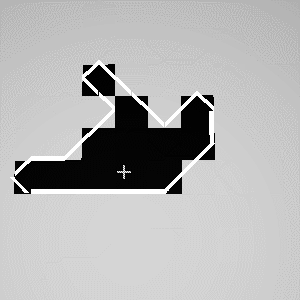
\includegraphics[width=.9\linewidth]{images/maps_0002}
  \end{subfigure}%
  \caption{Example room generation}
  \label{fig:room_generation_example}
\end{figure}

All objects in a room will be a part of a hierarchy. For example, dining chairs would be parented to a dining table, and a painting would be parented to a wall. To account for this kind of room structure, each room object will have its own list of specifications, which include its bounding box, a tag-based list of possible parents the object can have (e.g. a dining chair can be parented to a dining table), and a list of sides that children can place themselves against (i.e. top, bottom, left, right, front, and back).

 All of the bundle's room objects will try to find parents among themselves, which will include characters, items, furniture/props, and the room walls. Once a parent for a room object has been found, the object will try to align itself along one of the parent's sides, and if there is enough space, the object will position and orient itself beside the parent. If a parent is not found, a random position will be calculated that exists inside the room. A collision check will then be against the rest of the objects in the room, as well as against the room walls.

After the placement of all required room items of the bundle, additional side characters and items required for a scenario will be generated and added to the room using the same placement method as above to ensure there are no collisions or conflicts between characters, items, and furniture.

Once all the rooms have been created, they will then be connected to each other to allow traversal through each room in the map. Each of these connections will be represented in-game by a door item, which may be interacted with by the player in order to move between the different rooms in a layout.

\subsubsection{Furniture [essential]}
\label{sec:furniture_generation}
To ensure visual variability in the rooms of \ourgame, furniture will be procedurally generated at the beginning of every playthrough. To accomplish this, each type of furniture will be broken up into separate components. Multiple versions of these components, created in different styles, will be made. An example of components that would be used to make up a chair are its legs, seat, and back. These components will then be matched together with others using tags which dictate what furniture each component can be used in. The meshes of these components would then be joined to create one mesh to be used in the game. This will be done using the vertex manipulation capabilities of the engine.

\subsubsection{Characters [essential]}
\label{sec:character_generation}
The vast majority of characters in the world of \ourgame{} will be procedurally generated using a hierarchical component system which implies the natural hierarchy of a human skeleton. In this system, the human form is broken into 10 basic components: hands, lower arm, upper arm, feet, lower leg, upper leg, pelvis, torso, lower head, and upper head. Additionally, there are 4 face-detail components: eye, pupil, eyebrow, and nose. This component structure can be seen in Figure~\ref{fig:character_components}. Components which exist on both the left and right sides of the body may be asymmetrical, resulting in a potential total of 23 components. In order to achieve certain visual effects, components may be purposefully omitted from a character specification.

\begin{figure}[htb]
\centering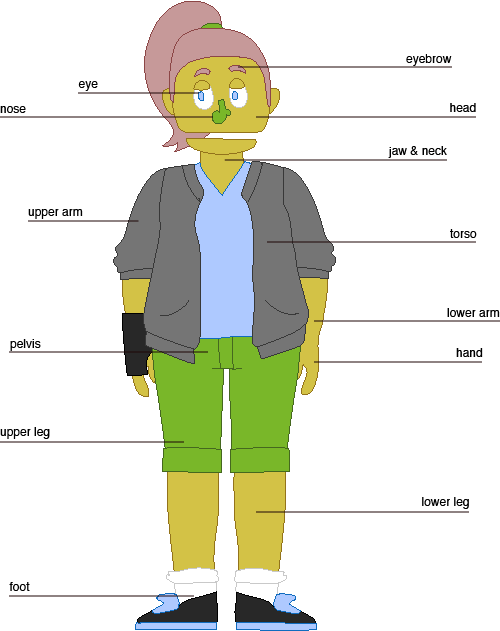
\includegraphics[width=.5\textwidth]{images/CharacterComponents}
\caption{Character Components}
\label{fig:character_components}
\end{figure}

In order to procedurally generate characters, a simple set of rules will be followed which result in the selection of individual assets for each component making up a single character. These rules are as follows:

\begin{enumerate}
\item{Limbs will always be selected as a whole, rather than as individual components. This is due to the difficulty involved in bridging the gap between the upper and lower limbs, i.e. the elbow and knee joints.}
\item{A component may optionally specify the selection of adjacent components.}
\item{All components must specify whether it is below or above its incoming component (this excludes pelvises, as they have no incoming components).}
\end{enumerate}

An example of this process can be seen in Figure~\ref{fig:character_generation_example}.

\begin{figure}[htb]
\centering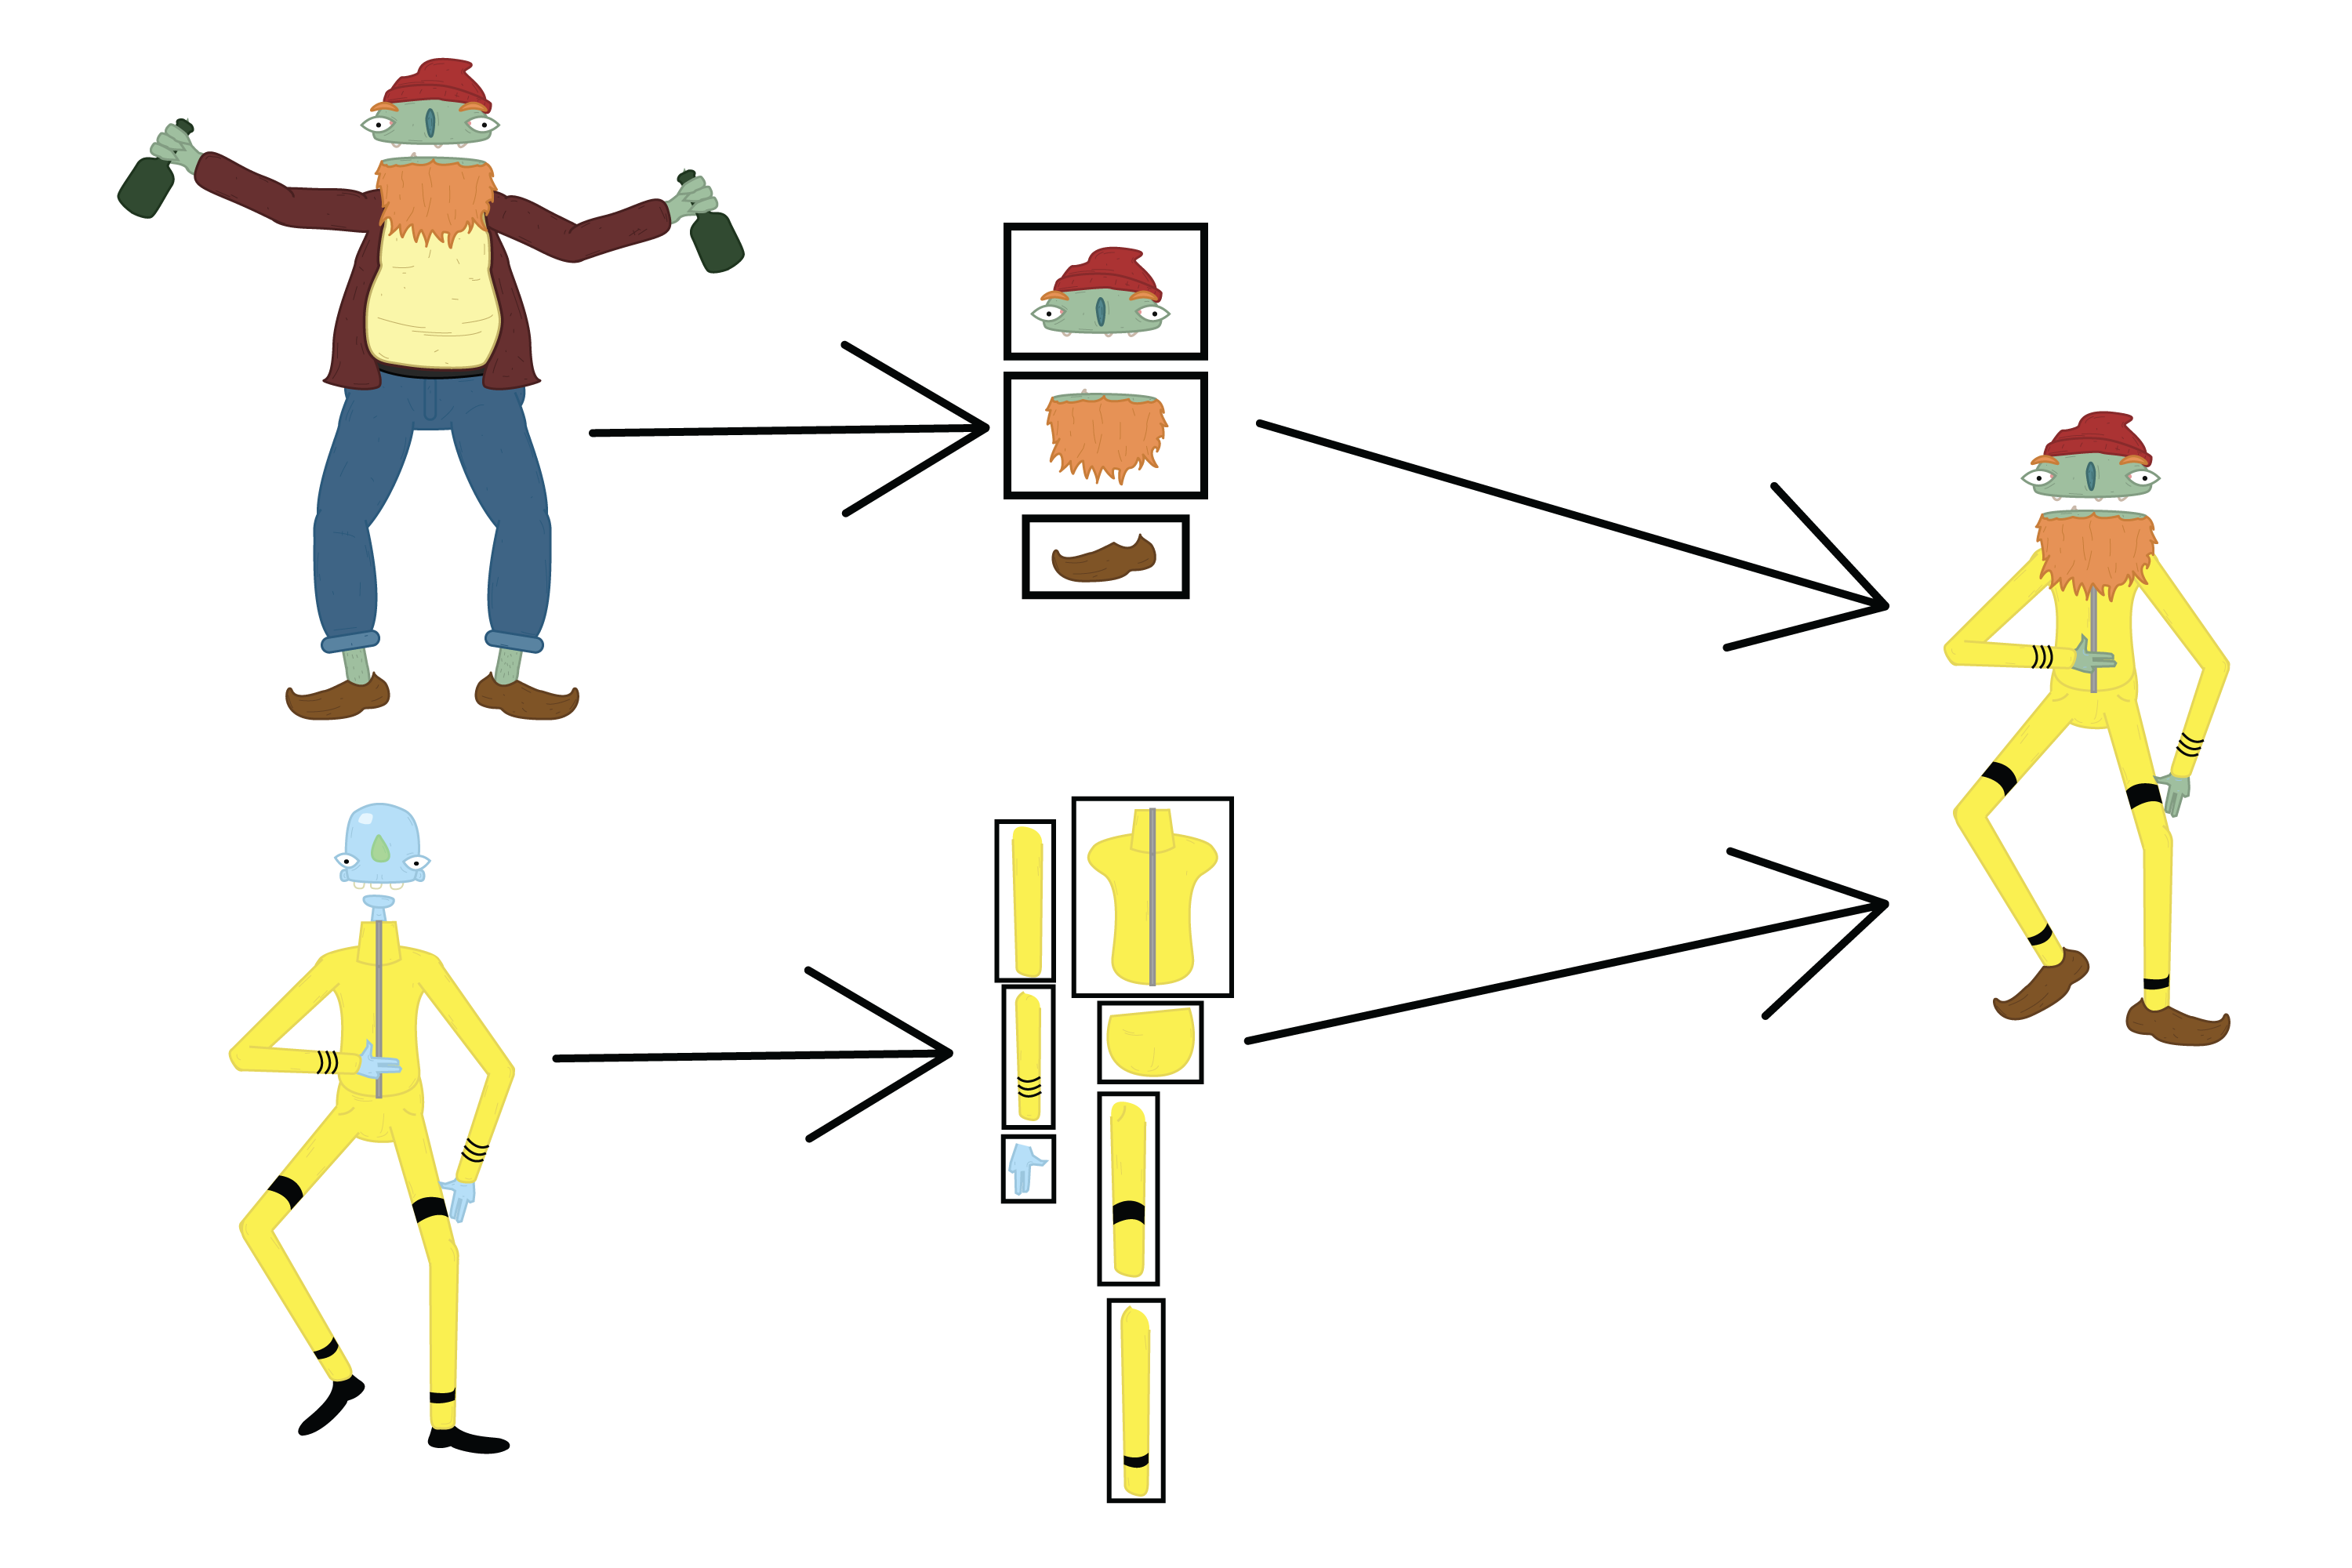
\includegraphics[width=.7\textwidth]{images/CharacterGeneration_Diagram}
\caption{Example character generation}
\label{fig:character_generation_example}
\end{figure}

\subsubsection{Audio [optional]}
\label{sec:audio_generation}
An audio clip of each note in an octave will be recorded and used for procedurally generating audio. When a song is created, a scale will be chosen, dictating which notes can  be used in a song. The notes can then be pitch shifted by octaves if desired. A time signature will also be chosen to effect the pacing of the song. The scale and time signature are dependant on the context of the room they will be placed in, taking into account the type of the room, and possible interactions within. To create more complex songs, songs with the same time signature but different scales can be layered along with simple percussion tracks. Multiple instruments will be recorded to add variety to the music that is able to be created.

\subsection{Scenario Editor [Planned]}
\label{sec:scenario_editor}
As the main plot of \ourgame{} requires the player to complete multiple playthroughs, it must be ensured that each playthrough is unique. If too much content is repeated, the player will lose interest. As room layouts are procedurally created, the generation algorithm must choose a series of scenarios to add to the rooms in a given playthrough. Each scenario can involve multiple characters, all with multiple lines of dialogue, multiple art assets, and different reactions depending on player input. To create the volume of content needed for this game, \ourteam{} will need to create an application that allows the team to quickly create formatted files that can be processed by \ourengine{} and added to the game world.

The Scenario Editor for \ourgame{} is intended to make it easy for \ourteam{}'s creative department to quickly create JSON files that contain all the information needed in a scenario. These files will be passed into the engine, which will read the data and add all the content to the game environment. The editor will have one tab for each of the main components of a scenario: characters, rooms, and dialogue. Each tab contains a list of the data necessary to create the object in the game world, with the ability to leave certain properties to be randomly determined by the engine. This allows the user to only fill in the information that is strictly necessary without having to curate every aspect of every in-game object.

The Characters tab allows the user to design characters for a particular scenario. The user can set basic information (age, gender, etc) as well as the states for the character at different points in the scenario. Each state is linked to a set of dialogue. For example, one scenario might consist of the player finding a character's lost item. The character would need at least two states: one default state, activated by default, which is linked to a dialogue where the character asks the player to find an item; and another state, activated by the player having the item stored in their inventory, which is linked to a dialogue where the player can tell the character that they have found the lost item. In the character tab, the user can also set which art assets should be used for the player. If no specific assets are set, the engine will randomly select which art assets to use for that character in the game.

In the Rooms tab, the user can design rooms for a scenario. The room data will include information about which characters and items can be found in the room. The user can give the room a "tag" - bathroom, or kitchen, for example - which will dictate what kind of furniture assets will be added to the room by the procedural generation system.

The Conversations tab will be where the user defines conversations between the player and any NPCs in a scenario. Each conversation can consist of multiple lines of dialogue, certain dialogue options from which the player can choose, and triggers to take the player into the yelling contest interface. Each line of dialogue must be set to a character in the Characters tab.

Once all the necessary data has been added, the user can save all the data into a set of JSON files. The files are saved onto the server, ready to be downloaded and used with \ourgame{}.



\subsection{File Management [Planned]}
Having the content generation system for \ourgame{} exist as a web application provides a number of advantages. The most significant advantage is that game scenarios will be stored online on the server, instead of being packaged with the base installation files for \ourgame{}. This will allow \ourteam{} to easily push new content and bug fixes to players after \ourgame{}'s official release. It will also make managing and testing content much easier during the development stage. In order to track changes and additions to the content, git will be packaged with \ourgame{}. The game will sync with a repository hosted on an external server, allowing players of \ourgame{} to efficiently receive content updates as soon as they are pushed to the remote repository.

\section{Target Audience}
\ourteam{}'s target audience for this project will primarily be the 18-29 age group. Reports from the PEW research center indicates that high percentages of this demographic are video game players and social media users. As this age group encompasses university students in most countries, there is a good chance that users have party experiences of their own to draw upon while playing \ourgame{}. 

Surreal individual experiences such as \textit{Crypt Worlds}, \textit{Slave of God}, and \textit{Proteus} have found success among users and critics alike by emphasizing exploration and discovery over more traditional game mechanics. \textit{Crypt Worlds} and \textit{Slave of God} have been featured in publications such as PC Gamer, Kill Screen Daily, Rock Paper Shotgun, and IndieGames.com. \textit{Proteus} has been nominated for and won numerous independent game awards, and was recently featured in the 2012 exhibit "Common Senses" at the Museum of Modern Art.
This type of contained single-player adventure focusing on storytelling has not only been successful in the freeware domain, but also has proven to be a commercially and critically successful formula. In February 2014, the creators of critically acclaimed and story-rich adventure \textit{Gone Home} announced their game had sold over 250,000 copies. The cultural trend is progressing toward more comedic and experimental forms of interactive storytelling when looking back through the history of video games. For example, \textit{Psychonauts}, which told an unconventional and humorous story, was a commercial failure at release. Since then, it has developed a large cult following and as of March 2012, has sold over 400,000 retail copies, not including sales from online platforms such as Steam and GOG.

In order to attract the attention of the target demographic, \ourteam{} will be creating a game following the current trend of experimental interactive experiences, providing the audience with unconventional gameplay and humour. As discussed above, these games, which stray from what is popular within the declining big budget video game industry as a whole, have seen great success.





\chapter{Tasks \& Deliverables}
Refer to Appendix~\ref{app:deliverables} for the full table describing \ourteam{}'s deliverables.

Refer to Appendix~\ref{app:wbs} for the full work breakdown structures.

Refer to Appendix~\ref{app:gantt} for the full Gantt charts.

% \subsection{Engine}
% The custom engine will have be yes good

% \subsection{Scenario Editor}
% The scenario editor will be presented as a server side web application. 

% \section{Content}
% A link to the repository containing the following assets will be provided.
% \subsection{Assets}
% All 2D art assets including characters and items will be saved without anti-aliasing. Character assets are generally comprised of twenty-three separate body components per character. The UI will also require certain assets such as the phone for the menu and backpack for inventory.
% All 3D art assets such as props and furniture pieces will also be included.
% \subsection{Scenarios}
% Written assets will be included as Json files, including descriptions for quests, character backstories, and player-character dialogue.

\section{Major Milestones}
\begin{figure}[htb]
\centering
\begin{tabular}{|l|l|}
\hline
{\bf Milestone} & {\bf Delivery Date}          \\ \hline
Prototype       & October 31st, 2015  \\ \hline
Alpha           & December 31st, 2015 \\ \hline
Beta            & February 29th, 2016 \\ \hline
Gold            & April 5th, 2016     \\ \hline
\end{tabular}
\caption{Milestone Dates}
\label{	Milestones Dates}
\end{figure}

\subsection{Party, Darling?}

\subsubsection{Prototype} 
\begin{enumerate}
\item Rigged controllable character
\item UI mockups for menu and inventory
\item 30 Character Designs
\item 36 Furniture Sets
\item 10 Static Props
\item 1 Song
\item Concept Art
\item Basic Random/Procedural Generation
\item Map Generator
\item Scenario Management System
\item Lattice Deformer
\end{enumerate}

\subsubsection{Alpha}
\begin{enumerate}
\item 60 Character Designs
\item 60 Furniture Sets
\item 30 Static Props
\item 3 Songs
\item Basic Sound Effects
\item Flare and Twist Deformer
\item Item Specification System
\item Completed AI
\item Character Interaction System
\item Final Menu UI and Character Interaction UI
\item Finalized Character Animations
\item Scripted Scene System
\item Item Interaction System
\item Local Save System
\item Status/Stats Management System
\item Inventory System
\item Door Travel System
\item Multiple Scenario Loader
\end{enumerate}

\subsubsection{Beta} 
\begin{enumerate}
\item 95 Character Designs
\item 35 Character Re-designs
\item 3D Model of Inter-mensional Room
\item 72 Furniture Sets
\item Additional Sound Effects
\item Introduction Written
\item Emotes
\item Promotional Website
\item Loading Screen Animation
\item Cloud Save
\item Yelling Mechanic UI
\item 7 Songs
\end{enumerate}

\subsubsection{Gold} 
\begin{enumerate}
\item 115 Character Designs 
\item 55 Redesigned Characters
\item 84 Furniture Sets
\item 40 Static Props
\item 9 Songs
\item Procedural Audio Generator
\item Finalized Side Quest Story Lines
\item Promotional Materials
\end{enumerate}

\subsection{S-Tengine2}
\subsubsection{Prototype}
\begin{enumerate}
\item Validate  existing systems(Ex. Scene Manager)
\item Lighting model improvements
\end{enumerate}

\subsubsection{Alpha}
\begin{enumerate}
\item Screen Space Ambient Occlusion
\item Positional Audio
\item Blinn and Phong Materials
\item Directional Light
\item Optimized UI System
\item Animation System
\end{enumerate}

\subsection{Scenario Editor}
\subsubsection{Prototype}
\begin{enumerate}
\item Django and Angular JS applications Created
\item Conversation Editor
\item Room Specification System
\item Character Builder
\end{enumerate}

\subsubsection{Alpha} 
\begin{enumerate}
\item Room Content Specification System
\item Component Tagging and Browsing
\item File Syncing
\end{enumerate}

\subsubsection{Beta}
\begin{enumerate}
\item Finalized UI
\end{enumerate}


\clearpage
\subsection{Documentation}
Several written documents will be completed corresponding with the senior project requirements.
\begin{enumerate}
\item Research Report - Early September
\item Project Plan - Early September
\item Peer Evaluation for Summer - Early September
\item Initial Design Document - Early October
\item Project Progress Presentation 1 - Late October
\item Final Design Document - Mid December
\item Peer Evaluation for Fall - Late December
\item Advisor Specific 1 - Late December
\item Project Progress Presentation 2 - Late January
\item Project Fair Plan and Promotional Material - Late February
\item Project Progress Presentation 3 - Late February
\item Project Fair - Early April
\item Peer Evaluation for Winter - Mid April
\item Advisor Specific 2 - Mid April
\item Project Closure - Mid April
\end{enumerate}

\chapter{Resources}
\section{Team Management}
\subsection{Management Policies}
\ourteam{} will be divided into two primary departments: creative and coding. For the duration of the project, leadership roles will be given to Michael Hetman, the Creative Director, and Ryan Bluth, the Lead Developer. For issues which fall within either the creative or coding domain, resolutions will be voted on by the members of the department. If there is an argument between two opposing sides, the side with the majority wins. In the case of an argument where the sides are equal, the leads of the department have the final say. For cross-domain issues, the department leads must make a decision together. If an agreement cannot be made between the Creative Director and the Lead Developer, Sean LeBlanc, as the most impartial, will cast the deciding vote.

\subsection{Team Structure}
\subsubsection{Ian Martin - Gameplay Goblin - Creative/Coding}
\begin{tabular}{m{0.15\linewidth} m{0.8\linewidth}}
\raisebox{-\linewidth}{\includegraphics[width=\linewidth]{images/Ian}} & Ian will be in charge of designing \ourgame{}'s narrative. This will include researching and developing in-house tools for generating and integrating content into the game. As a narrative designer, Ian will ensure story and gameplay elements work together to enhance the player experience. Ian is also an independent musician, and will help to contribute audio for the game.\\
\end{tabular}

\subsubsection{Ryan Bluth - Programophile - Coding}
\begin{tabular}{m{0.15\linewidth} m{0.8\linewidth}}
\raisebox{-\linewidth}{
\includegraphics[width=\linewidth]{images/Ryan}} & Ryan will be spearheading the server-side development of \ourgame{}'s web components. Additionally, Ryan will be developing many aspects of \ourteam{}'s in-house engine and will use his experience in game design to help create the scenario editor and gameplay mechanics.\\
\end{tabular}

\subsubsection{Michael Hetman - Audio-Visual Disaster - Creative/Coding}
\begin{tabular}{m{0.15\linewidth} m{0.8\linewidth}}
\raisebox{-\linewidth}{
\includegraphics[width=\linewidth]{images/Michael}} & Michael will be the creative lead for the 3D assets in \ourgame{}, with his work primarily consisting of environment and prop modelling, as well as texturing and overall design. In order to make the production of 3D assets more efficient, Michael will also be working on scripts which allow for procedural generation of simple models for use in the game. Michael will also support the art department by working on additional 2D art assets when available. As an experienced independent musical disaster, Michael will additionally apply his talents to the composition of audio for the game.\\
\end{tabular}

\subsubsection{Sean LeBlanc - Syntax Swammi - Creative/Coding}
\begin{tabular}{m{0.15\linewidth} m{0.8\linewidth}}
\raisebox{-\linewidth}{\includegraphics[width=\linewidth]{images/Sean}} & Sean will be the lead systems developer on \ourgame{}. Sean has contributed much to \ourteam{}'s in-house game engine and the knowledge gained from his work will transfer to systems development throughout the development of \ourgame{}. Sean has also worked on a number of games as both a programmer and an artist, which will allow him to contribute to the development of gameplay and 2D art assets.\\
\end{tabular}

\subsubsection{Emma Thurlow - Code Whisperer - Coding}
\begin{tabular}{m{0.15\linewidth} m{0.8\linewidth}}
\raisebox{-\linewidth}{
\includegraphics[width=\linewidth]{images/Emma}} & Emma will be focusing on programming specific gameplay elements and mechanics. Emma will also be helping to design and develop the server-side application. Emma has experience developing games from other projects as well as web design experience, and these skills will transfer over to the development of \ourgame{}.\\
\end{tabular}

\subsubsection{Catherine Wong - Mere Dilettante - Creative}
\begin{tabular}{m{0.15\linewidth} m{0.8\linewidth}}
\raisebox{-\linewidth}{
\includegraphics[width=\linewidth]{images/Cat}} & Catherine has been an illustrator on various other projects and will be assuming a similar role on \ourgame{} as the lead 2D artist. She also has experience working with 3D models, and will help to model and texture the environments in the game. Additionally, she will be lending her creative talents to the game's narrative design.\\
\end{tabular}




\section{Hardware}
\subsection{Computer}
In order to run \ourgame{}, a relatively powerful personal computer will be required. The computer will require at least 16 gigabytes of RAM, an Intel Core i7 processor or equivalent with a clock speed of at least 3.0 gigahertz, and a graphics card with a clock speed of at least 1.0 gigahertz, at least 2 gigabytes of memory, and support for OpenGL 3.3.

\subsection{Server}
Due to the fact that the content creation service is online, access to a remote server will be required. External access will be achieved using a Secure Shell Connection (SSH). This will allow \ourteam{} to configure the server to run the Scenario Editor web application described in Section~\ref{sec:scenario_editor}.

\subsection{Projector}
A projector may be used when demonstrating \ourgame{} at the senior project fair. This will allow for a larger display of \ourgame{}. In order to make the use of a projector, a proper projecting surface will also be required.

\section{Software}
\subsection{Visual Studio 2012/2013}
\ourengine{} projects, and by extension \ourgame{}, are developed in C++. Of the many options available for C++ development, \ourteam{} has decided to make Visual Studio the team's standard IDE for both engine and gameplay programming. Visual Studio is offered by Microsoft for free and is already installed on university computers, giving team members access to the software whenever they need it.

\ourteam{} plans to take advantage of some of Visual Studio's project management tools in order to make development across many different projects and environments easier. In particular, the creation of standardized project property sheets, which are shared between different solutions, will allow many of the more arcane and difficult setup tasks to be automated.

\subsubsection{VCProjer}
In addition to Visual Studio's built-in tools and features, \ourteam{} will develop a custom command-line interface which makes development using both the 2012 and 2013 versions of Visual Studio a fairly seamless process. As the 2013 project files are not backwards compatible with Visual Studio 2012, both versions must be maintained in order to transfer between different development environments. VCProjer will make the file management necessary for maintaining the two different project versions much simpler by copying file inclusions from one version to the other during builds.

\subsection{Adobe Photoshop \& Illustrator}
\ourteam{}'s art department will be performing the majority of their 2D artwork in Adobe Photoshop and Illustrator. All members of the team are experienced with Adobe software, and are comfortable using these tools in their workflow. Adobe Illustrator is tailor-made for producing vector graphics, and as such will be used for assets which may require variable resolution. Adobe Photoshop will be used for editing raster assets.

\subsection{Autodesk Maya}
\ourgame{}'s 3D assets, such as props and furniture pieces, will be created in Autodesk Maya, a 3D modelling and animation suite. Maya was chosen over other similar programs for many reasons. Due to the art department's familiarity and experience with the system, Maya will allow for a faster workflow. Also, since Maya is installed on all lab computers and is free to download, it is also the most accessible software for the team. It also provides the required functionality, such as exporting meshes as obj files, and creating prototype scripts in python. 

\subsection{GitHub app \& Atlassian SourceTree}
\ourteam{} plans to use git (specifically public GitHub repositories) for file management. In lieu of interfacing with the git repositories solely through command line tools, the team will also make use of simple GUI wrappers for git commands. \ourteam{} will use GitHub's app for basic git commands such as pulling/pushing changes, merging branches, etc., and also SourceTree, in order to gain access to more advanced git commands in addition to the ones made available by GitHub.

\subsection{\LaTeX{} \& Overleaf}
For official project documentation, \ourteam{} will be using Overleaf, a collaborative writing environment which uses the \LaTeX{} markup language. In addition to offering a collaborative writing environment similar to Google Docs, Overleaf also automatically stores a history of changes made to individual documents and allows the team to flag specific versions for preservation.

Although the team has limited experience with \LaTeX{}, it is anticipated that the strict separation of content and presentation will make the creation of standard project documentation much more efficient. The process for writing multiple documents spanning a large number of pages using a more common word processor, such as Google Docs or Microsoft Word, would be an arduous task. Applying consistent design principles to each would require \ourteam{} to spend a significant amount of time manually formatting text throughout the entire document. The use of \LaTeX{} will allow the team to create one or two shared document classes that manage the presentation of content, allowing team members to spend more time focusing on writing content without a concern for presentation.

\subsection{HipChat \& ProBoards}
Additional software that will be used will include tools for project management and collaboration. HipChat by Atlassian, a private group chat service, will be used as a method of communication for the team where all room conversations are archived and easily searchable. A private discussion board provided by ProBoards will be used to permanently log the team's research, ideas, meeting notes, and other collaborative content.


\chapter{Risk Management}
\section{Estimated Risks}
In order to determine an estimated probability for the loss of a team member, the potential reasons for absence were listed and assigned a percentage value. \ourteam{} estimated that the base probability rates for illness, mortality, or becoming otherwise incapacitated by reviewing Canadian statistics and selecting values marginally above the given rates. The values used in the final estimations are presented in Figure~\ref{fig:risk_base_percentages}.

\begin{figure}[htb]
\caption{Base Estimations for Risk Analysis}
\label{fig:risk_base_percentages}
\centering\begin{tabular}{| c | c | c |}
\hline
Reason of Absence & Time Away & Probability\\ \hline
Illness & 1 week & 16\% (individual)\\ \hline
Illness & 1 month & 4\% (individual)\\ \hline
Illness & 1 year & 1\% (individual)\\ \hline
Immediate Crisis & 1 week & 1\% (per potential crisis)\\ \hline
Extended Crisis & 1 month & 1\% (per potential crisis)\\ \hline
\end{tabular}
\end{figure}

In addition to the base risk percentages, individual team members are known to be at a higher risk for various other factors. Ryan Bluth has recently became aware of an acute illness, thus the probability of his absence has been increased by 10\%. Similarly, there is a 1\% chance that Michael Hetman will leave in order to start a family, and his risks have been adjusted accordingly.


\section{Risk Analysis}

In order to determine relevant risks, the probability of individual members being absent during the project was multiplied by the impact (the estimated percentage of the project which would be lost as a result of their absence). This product is the \textbf{exposure} for the given risk and time period. The calculated exposure value, along with the planned corrective action for loss is presented in Figure~\ref{fig:risk_analysis}.

In addition to the risk of losing individual team members, certain combinations of absence require specific corrective actions, typically because the corrective action for losing one involved reassigning tasks to the other. These cases are presented in Figure~\ref{fig:risk_analysis_pairs}.

\begin{figure}[htb]
\caption{Risk Analysis}
\label{fig:risk_analysis}
\centering\begin{tabular}{|p{0.07\textwidth}|p{0.07\textwidth}|p{0.075\textwidth}|p{0.05\textwidth}|p{0.07\textwidth}|p{0.5\textwidth}|}
\hline
Team member & Length of Absence & Probability & Impact & Exposure & Corrective Actions\\ \hline
%
\multirow{3}{*}{Ryan} & 1 week & 56\% & 1\% & 0.56 & Lose time on bug testing\\ \cline{2-6}
 & 1 month & 22\% & 15\% & 3.3 & Depth mapped shadows not included in the lighting model\\ \cline{2-6}
 & 1 year & 6\% & 40\% & 2.4 & Lose all optional features (inventory, multiple monitor support, categorized volume controls), character recruiting and yelling contests\\ \hline
%
\multirow{3}{*}{Emma} & 1 week & 23\% & 1\% & 0.23 & Lose procedurally generated item descriptions, they will be manually written instead\\ \cline{2-6}
& 1 month & 7\% & 10\% & 0.7 & Lose nested hierarchy furniture procedural generation. Reduce types of rooms that can be procedurally generated\\ \cline{2-6}
& 1 year & 1\% & 35\% & 0.35 & Lose all optional features, lose character recruiting feature and yelling mechanic. Lose procedural house layout system, rooms are destroyed when player leaves, no backtracking.\\ \hline
%
\multirow{3}{*}{Sean} & 1 week & 36\% & 1\% & 0.36 & Lose time on bug testing\\ \cline{2-6}
& 1 month & 10\% & 8\% & 0.8 & Lose facial rigging in character animation feature, emotes, multiple monitor support, categorized volume control\\\cline{2-6}
& 1 year & 1\% & 40\% & 0.4 & Lose all optional features, character recruiting feature and yelling mechanic\\ \hline
%
\multirow{3}{*}{Michael} & 1 week & 35\% & 2\% & 0.7 & Lose a small amount variety in 3D assets\\ \cline{2-6}
& 1 month & 5\% & 10\% & 0.5 & Basic low detail furniture and props will be non-uniformly scaled for variation in lieu of being procedurally generated\\ \cline{2-6}
& 1 year & 2\% & 30\% & 0.6 & Lose procedural generation of all furniture and props, and procedural audio generation of background music\\ \hline
%
\multirow{3}{*}{Ian} & 1 week & 41\% & 2\% & 0.82 & Decrease amount of side-quest ideas\\ \cline{2-6}
& 1 month & 7\% & 10\% & 0.7 & The scenario editor web application will not be styled for visual appeal. Lose the procedural insult generator, insults will be manually written instead.\\ \cline{2-6}
& 1 year & 1\% & 30\% & 0.3 & Scenario editor and writing tasks will be delegated to Catherine. Number of scenarios, characters and items will be halved.\\ \hline
%
\multirow{3}{*}{Catherine} & 1 week & 35\% & 1\% & 0.35 & Lose 5 characters, 2 items\\ \cline{2-6}
& 1 month & 7\% & 7\% & 0.49 & Lose 20 characters and 8 items\\ \cline{2-6}
& 1 year & 1\% & 30\% & 0.3 & Art asset tasks will be delegated to Ian. Number of scenarios and characters will be halved. Lose all unfinished items.\\ \hline

\end{tabular}
\end{figure}


\begin{figure}[htb]
\caption{Risk Analysis (Pairs)}
\label{fig:risk_analysis_pairs}
\centering\begin{tabular}{|p{0.14\textwidth}|p{0.075\textwidth}|p{0.05\textwidth}|p{0.07\textwidth}|p{0.5\textwidth}|}
\hline
Team members & Probability & Impact & Exposure & Corrective Actions\\ \hline
Ryan \& Sean - Engine Developers & 0.06\% & 45\% & 0.027 & Lose engine. Emma, Ian, and Michael will become main programmers. They have a bit of experience in Unity and will switch engines. Switch to sprite-based character animation. In addition to their individual lost features, lose procedural character generation. Menu options are added back because of Unity support. Drop file management (server system).\\ \hline
Catherine \& Michael - Primary Artists & 0.02\% & 40\% & 0.008 & A lot of characters and content would need to be scrapped, and Sean and Ian would take over the 2D and 3D art. Because they would need to put more focus towards artwork, game features would be lost. These features would be all optional game features, half of the scenarios, and any styling of the scenario editor.\\ \hline
Ian \& Catherine - Narrative Designers & 0.01\% & 35\% & 0.0035 & Michael and Sean would take over the art creation. As a consequence, half of the procedural furniture would be scrapped along with the variation of furniture generated. All optional game features would also be scrapped.\\ \hline

\end{tabular}
\end{figure}


\chapter{Change Control Policy}
\label{ch:change-control-policy}
\section{GitHub Repositories}
\ourteam{} has been committed to open source development since its founding, and intends to keep this mindset throughout the development of \ourgame{}. To this end, public GitHub repositories will be used for file storage and version control. \ourteam{} will also be taking advantage of GitHub's "Organizations" feature, which aggregates a team of users under a single umbrella account. This allows team members to switch to a single unified context while working on GitHub in order to focus on the project.

To simplify development, large projects will be given their own individual repository under \ourteam{}'s name. Individual repositories are planned for the game engine, for the scenario editor, and for \ourgame{} itself. Two additional general-purpose repositories are planned for art assets and documentation. More repositories may be added during development should the need for further decentralization arise.

\section{SweetHeart Sitdowns}
\textit{"SweetHeart Sitdowns"} is the private discussion board for \ourteam{}. It is primarily used for communication and documentation. Using the board's file storage capabilities, materials used to supplement documentation are stored here so they can be easily referenced along with their related notes. These files can include figures, concept art for group review, and reference materials. When these files are ready to be incorporated into \ourgame{} or the associated public documentation, they will be transferred to storage in the appropriate GitHub repository.

\chapter{Communication Policy}

\section{Meetings}
\label{sec:meetings}
As with any project, the development of \ourgame{} involves several group discussions in which team members can brainstorm, collaborate, discuss issues, etc. In order to ensure that they are an efficient and effective use of time, all scheduled meetings will follow a basic pre-defined structure. Each will begin with a quick overview from each member on their task progress since the last meeting, followed by a group discussion of new ideas and how they would or would not fit within \ourgame{}'s narrative. After this, agenda items written prior to the meeting will be addressed and take up the bulk of the meeting time. The last few minutes of meetings will be reserved for new assignments, in which group members are each assigned new or previously unfinished tasks to work on until the next meeting.

In order to keep team members focused and productive over the course of extended meetings, breaks will be included in the form of semi-scheduled "review sessions" in which the group play videogames together and then discuss their success and cultural significance (or lack thereof). In particular, the group will attempt to review games which implement mechanics or elicit player reactions similar to those planned in \ourgame, and apply these observations to the development process.

Notes are taken during each meeting for documentation purposes. These notes are posted on the private discussion board described in Section~\ref{sec:forum}. 

\section{HipChat}
\ourteam{}'s primary channel for communication will be a private group chat provided by Atlassian's HipChat service. This chat service will provide the team with access to multiple chat rooms with a fully searchable history. \ourteam{} intends for the use of HipChat to serve as a professional alternative to common instant messaging services (Facebook, mobile texting, etc). 

In addition to basic chat functionality, HipChat offers many useful features and integration opportunities which \ourteam{} plans to take advantage of throughout the development of \ourgame{}. A GitHub integration will be established to automatically post HipChat messages whenever changes are pushed to \ourengine{}'s repository. This will allow team members working on other portions of the project to stay up-to-date on engine progress. A similar integration has been put in place to notify the group about status updates on GitHub issues. HipChat allows users to upload files and send them to other users, however, in accordance with the file management policy described in Section~\ref{ch:change-control-policy}, \ourteam{} has decided that this should only be used for simple file transfer and sharing of assets and should not be treated as a replacement for storage or relied upon for file hosting.

Custom HipChat functionality will also be implemented in the form of a group chatbot deployed as an external Heroku application. To control this chatbot, the team will be able to ping it directly or set up periodic interactions through cronjobs, and is currently used to manage group reminders.


\section{SweetHeart Sitdowns}
\label{sec:forum}
Although HipChat is a very useful tool for direct communication, it is not intended to replace formal documentation, and the student package \ourteam{} plans to use has limitations on the amount of chat history that can be preserved. In order to provide members with a more structured and persistent channel for documentation and communication, \ourteam{} will also maintain \textit{"SweetHeart Sitdowns"}, a private discussion board hosted through the ProBoards service.

As described in Section~\ref{sec:meetings}, notes taken during meetings are posted to the discussion board in order to provide team members with reliable time-stamped documentation of team discussion, decisions, and progress made.

The discussion board is also used for internal management of group policies and individual member status. For example, during the summer research period, \ourteam{} created a policy which prescribed a set of rules to the development of concept art. Under the terms of this policy, every member of the art department was tasked with creating at least one fully illustrated piece of concept art for a potential character in \ourgame{}, as well as provide a few short details about their existence in the game world (name, reason for being at the party, etc). In order to enforce and evaluate the effectiveness of this policy, the work created by individual artists was all posted to the discussion board. Upon review at weekly meetings, notes were edited into the individual character posts providing constructive criticism and pointing out any noteworthy details which the team enjoyed.

Another example of the use of the discussion board for internal management from the summer research period was the maintenance of project development blogs as forum threads. Each week, every member of \ourteam{} would post an update to a project-specific thread explaining any significant progress made since the last update in order to provide an ongoing record of the project's status. This was particularly useful for projects which were a collaborative effort between multiple team members, as it allows developments made by one member to be easily shared among the rest of the group.

Throughout the development of \ourgame{}, \ourteam{} will be working on secondary projects which will use \ourengine{}. To manage these, a side project forum will be created where group members can discuss and coordinate these individual projects.

\chapter{Quality Control Policy}
\section{Gameplay}
In order to ensure that the gameplay of \ourgame{} is of high quality, \ourteam{} will perform bi-weekly user testing with a number of users. These users will have varying levels of videogame experience which will provide a more diverse set of criticism. By performing these tests on a bi-weekly basis \ourteam{} will be able to react more quickly to deficiencies in the gameplay of \ourgame{}. 



\section{Optimization}
As \ourteam{} is developing a custom engine with little industry experience, unforeseen performance and design issues are a potential risk. To help avoid and prevent these issues, the engine developers will research existing methods before adding to or refactoring parts of \ourengine{}. This will also help to ensure that the engine features are efficient and effective. 

In order to evaluate the performance of various engine features, \ourteam{} will be making use of Visual Studio's performance analysis tools. These tools generate comprehensive reports breaking down the use of computation cycles within given processes and functions. In particular, they may be used to isolate the call tree which accounted for the largest number of computation cycles during the profiling session. This feature can be used to identify engine bottlenecks and high-cost functions and help the engine programmers to focus on problematic code.

\section{UI}
Players may be unable to comprehend the user interface in \ourgame{}, which can cause them to miss important elements of the game. This could lead to increase of frustration and negatively impact their overall game experience. Throughout development, the user interface will need to be tested on people who are not familiar with gaming. The user interface will be re-designed according to feedback from novice users collected during testing.

The current design of the inventory system uses natural sorting, allowing players to place objects spatially in the backpack interface. Although this method is quite analogous to the real-world experience of using a backpack, the screen space in the inventory UI may become cluttered easily. Because of this, players may not be able to easily sort through and find inventory items, leading to frustration. To prevent excessive clutter in the inventory UI, scenarios and procedural room generation will need to incorporate a generally small amount of items. Only quest specific items and a minimal amount of random items will be placed in the environment. If user testing results find that the inventory system needs to be improved, \ourteam{} may forgo the original style and redesign the backpack UI to be explicitly organized, though it may feel less natural (and thus less immersive) to the player.

\section{2D + 3D}
The decision to incorporate both 2D and 3D art together in the intended fashion is uncommon among similar first person point-of-view games, and the dissonance between the two mediums may be significantly jarring for players, leading to possible breaks in immersion during gameplay. The difference between 2D and 3D art elements is not merely an artistic decision, and is intended to function as a means to differentiate between interactive and non-interactive elements in the game. Consistency will be crucial when creating the art assets, ensuring that all interactive elements are 2D and all non-interactive elements are 3D. By adhering to this principle of differentiation, \ourteam{} hopes to take advantage of the apparent dissonance in order to communicate these game mechanics to the player.

If user testing results show that the purposefully clashing combination of 2D and 3D elements in \ourgame{} is too disorienting for players, \ourteam{} will need to compromise the original artistic vision in order to incorporate more stylistic similarities between the 2D and 3D elements. To do this, the depth and detail of 3D meshes may be decreased, and the implied depth in the illustration of the 2D elements may be increased. Additionally, the lighting model used in the environment shaders may be modified such that it more closely resembles the flat, cell-shaded look of the 2D elements. This may make the differentiation between interactive and non-interactive objects more difficult, which may require further changes to UI to ensure players are not confused.

\section{Multiple Artists}
As the character art assets are being developed by multiple members of \ourteam{}, the differences between each artist's preferred art style may cause the art assets to be visually incompatible. In order to evaluate how effectively each artist's assets match the game's intended art style, surveys will be conducted with potential players. During these surveys, participants will be presented a selection of assets from all artists, without knowing which artist designed which asset. Participants will be instructed to group the assets by their assummed creator, explaining the reasons for their grouping. An example of the survey tools are shown in Figure~\ref{fig:survey}.

\begin{figure}[htb]
\centering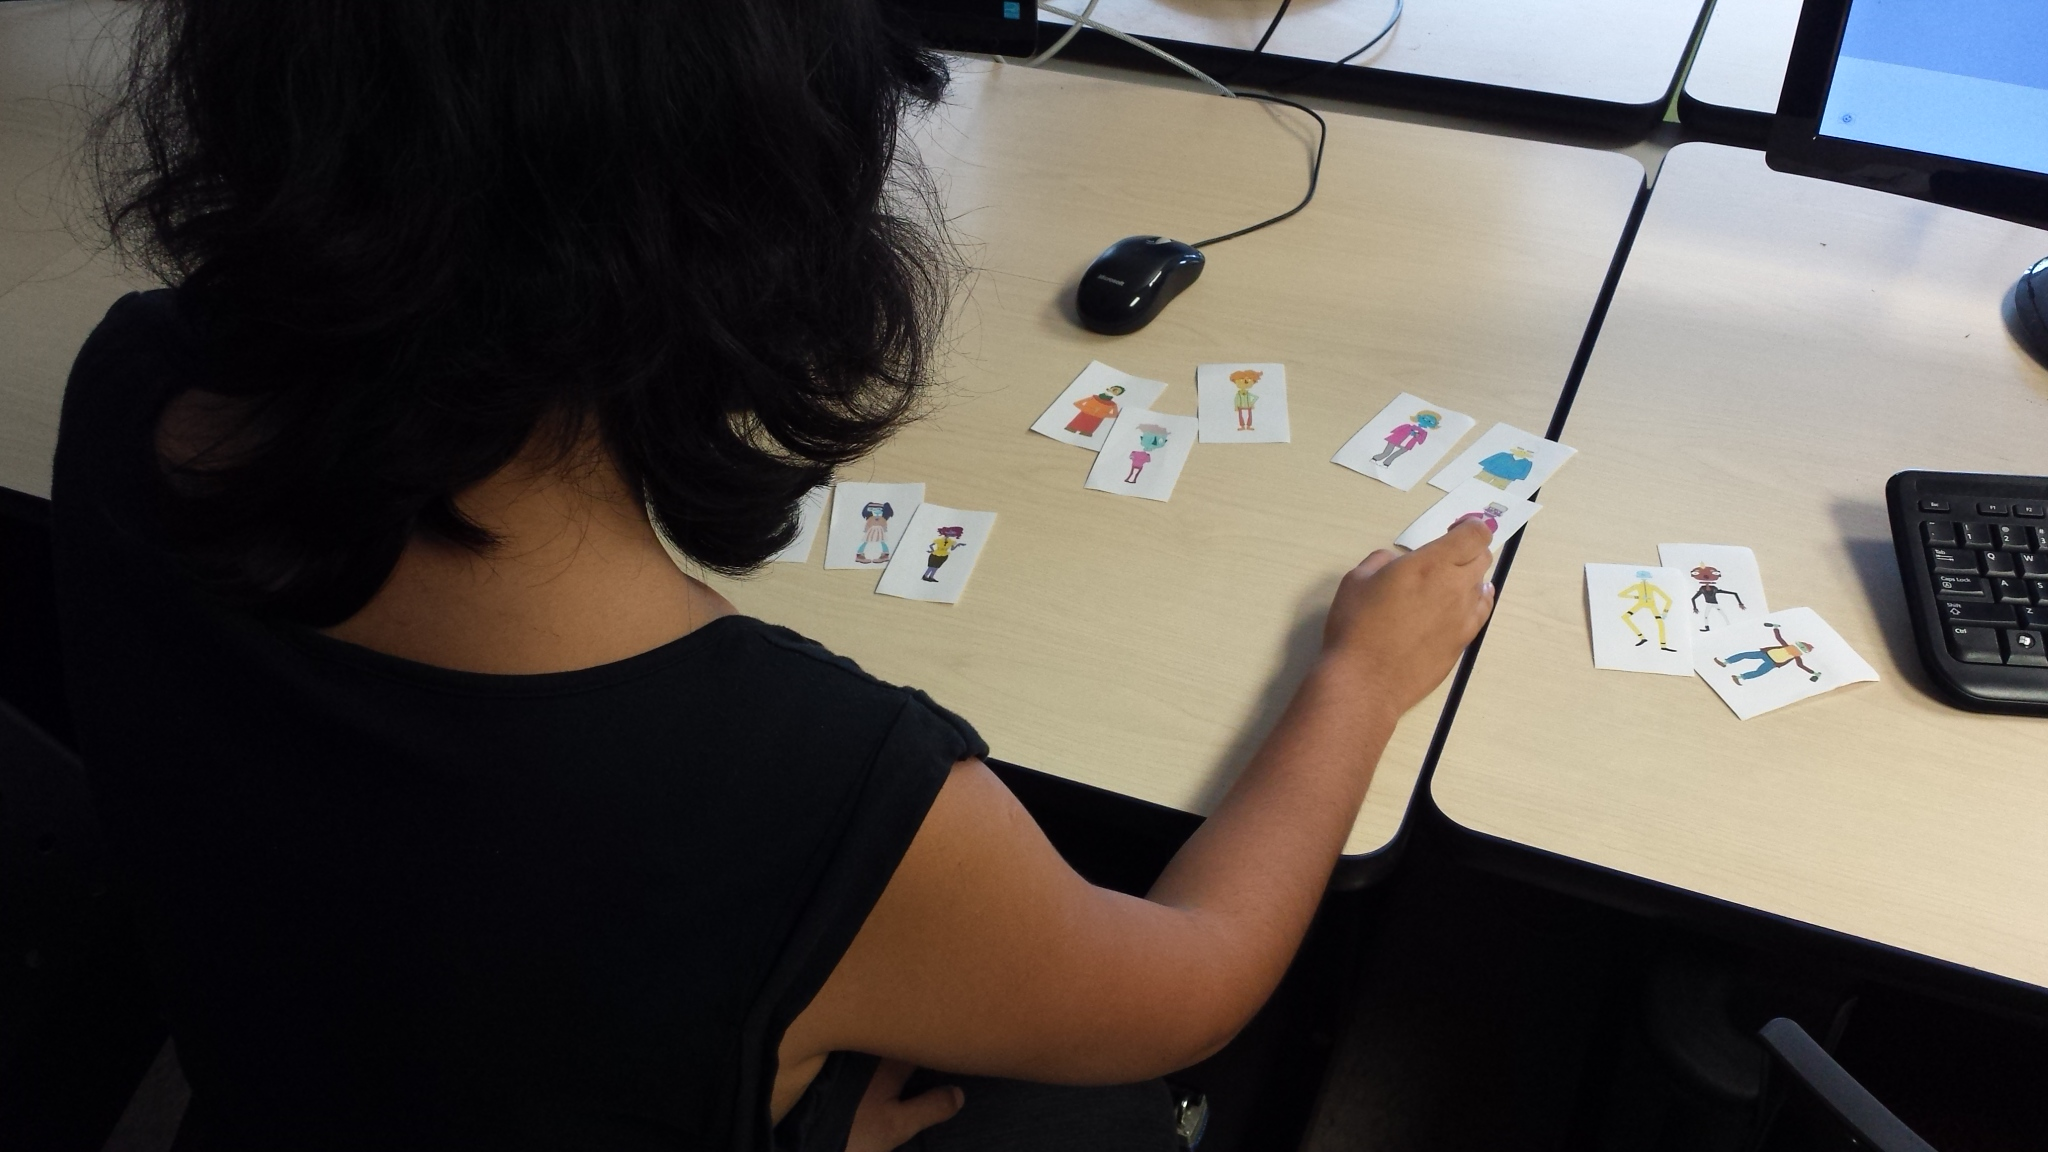
\includegraphics[width=.7\linewidth]{images/ArtisticCohesion}
\caption{Artistic Cohesion Survey Tools}
\label{fig:survey}
\end{figure}

If participants are able to correctly place assets created by a single artist in the same group, and provide one or more logical reasons for their grouping, this may indicate that the artist has failed to match the intended vision. Together, the artists can evaluate the feedback and attempt to identify and ameliorate the visual elements that participants feel are jarring or out-of-place.

\chapter{Marketing}

In order to spread the word of \ourgame{}, \ourteam{} will enact various marketing strategies throughout development.

\section{Social Media}

Due to the popularity of social media and its ability to bring people with similar interests together, \ourteam{} has created a number of social media accounts to connect with their target audience, providing a behind-the-scenes look at the game's development.

\subsection{tumblr}
Every week a member of \ourteam{} will write a post on the team's tumblr blog incorporating figures and images from the development process. This post will describe what aspects of the game the team is currently working on, and discuss upcoming features and plans. Through this account, \ourteam{} also hopes to follow and connect with other game developers and development teams.

\subsection{Twitter}
Twitter will be used to share short announcements pertaining to \ourteam{}. Announcements can include reaching large milestones for \ourgame{}, as well as side projects and events the team is participating in. The Twitter account can repost relevant tweets that individual members have posted to their own Twitter accounts. Gameplay and development videos created with the Vine app can also be posted. In the future, it can be used as a way to directly communicate and exchange ideas with the userbase of \ourgame{}.

\subsection{Facebook}
Facebook will be used near the end of development in order to inform the friends and family of \ourteam{} members of the upcoming project fair. Friends and family will be encouraged to share posts with their own contacts to increase the reach of this information.

\section{Live Events}
\ourteam{} will be participating in various game jams throughout the year to hone their development skills and to grow together as a team. At these events, they will have the opportunity to show off \ourengine{} to generate interest. Members of \ourteam{} will also attend local developer meet-ups, such as Dirty Rectangles, to network and discuss game development.

\section{Website}
In preparation for the Senior Project fair, a promotional website will be created by members of \ourteam{}. This website will include an overview of the game's story, mechanics, and features. The site will include a trailer for \ourgame{} and a biography for each member of the team.

\section{Promotional Materials}
Game posters will be designed and posted to promote the game's unveiling at the 2016 IMD Senior project fair. Additionally, chocolates will be distributed outside the project demonstration, and will be shaped into the form of \ourteam{}'s logo using molds the team will produce with the help of a 3D printing service.

\appendix
\chapter{Appendix - Deliverables}
\label{app:deliverables}
Includes deliverables for the Scenario Editor, \ourengine{}, and \ourgame{}.
\BgUsefalse % deactivates background
\includepdf[fitpaper=true]{ProjectPlan_Deliverables.pdf}
\BgUsetrue % deactivates background

\chapter{Appendix - Work Breakdown Structures}
\label{app:wbs}
Includes work breakdown structure diagrams for the Scenario Editor, \ourengine{}, and \ourgame{}.
\BgUsefalse % deactivates background
\includepdf[fitpaper=true]{webStuffTasks.pdf}
\includepdf[fitpaper=true]{S-Tengine2Tasks.pdf}
\includepdf[fitpaper=true]{GameTasks.pdf}
\BgUsetrue % activates background

\chapter{Appendix - Gantt Charts}
\label{app:gantt}
Includes Gantt charts for the Scenario Editor, \ourengine{}, and \ourgame{}.
\BgUsefalse % deactivates background
\includepdf[fitpaper=true]{ScenarioEditor.pdf}
\includepdf[fitpaper=true]{S-Tengine2Gantt.pdf}
\includepdf[fitpaper=true]{GameGantt.pdf}
\BgUsetrue % activates background

\end{document}